\chapter{Statistica bosonica e fermionica}
Si consideri prima di tutto un sistema classico di particelle identiche non interagenti la cui funzione di partizione, tenendo conto del fattore di Gibbs, è data da
\begin{equation}
    Z_{(N)} = \frac{1}{N!}Z_{(1)}^N, \quad Z_{(1)} = \nsum_{a}e^{-\beta\epsilon_a} \equiv \nsum_\epsilon e^{-\beta\epsilon}.
\end{equation}
Usando l'espressione \eqref{eq: funzione di partizione grancanonica (fugacità)}, la funzione di partizione grancanonica è data da
\begin{equation}
    Q_{C} = \nsum_Nz^NZ_{(N)} = \nsum_N\frac{1}{N!}(zZ_{(1)})^N = e^{zZ_{(1)}},
\end{equation}
per cui il potenziale grancanonico è
\begin{equation}
    \varpi_{C} = -\frac{\log{Q_{C}}}{\beta} = -\frac{z}{\beta}Z_{(1)}.
\end{equation}
Usando la \eqref{eq: numero medio N (grancanonico)}, si può ricavare il numero medio di componenti 
\begin{equation}
    \vmedio{N}_{C} = zZ_{(1)} = \nsum_\epsilon ze^{-\beta\epsilon} = \nsum_\epsilon e^{-\beta(\epsilon - \mu)}.
\end{equation}
D'altra parte, il numero medio di componenti è anche determinato dalla somma del numero medio di particelle $n(\epsilon)$ in ogni livello $\epsilon$, per cui
\begin{equation}
    \vmedio{N}_{C} = \nsum_\epsilon \vmedio{n(\epsilon)}_{C}.
\end{equation}
Dal confronto di queste due espressioni per $\vmedio{N}_{C}$ è immediato trovare che
\begin{equation}
    \vmedio{n(\epsilon)}_{C} = e^{-\beta(\epsilon - \mu)} = ze^{-\beta\epsilon}.
\end{equation}
Dunque, secondo l'approccio classico il valore medio del numero di particelle per livello decresce in maniera esponenziale. 

\section{Gas ideale di bosoni}
Si consideri ora il medesimo sistema di particelle identiche non interagenti ma descritto tramite l'approccio quantistico supponendo che le componenti di tale sistema siano bosoni. In questo caso, ogni microstato $\nu$ è caratterizzato solamente da quante particelle in ciascuno dei possibili livelli di energia $\epsilon$ del singolo componente, indipendentemente da quali di queste; quindi, $\nu$ è determinato dai numeri di occupazione $n(\epsilon)$, con $n(\epsilon) \in \N_0$, senza alcuna limitazione in quanto il numero totale di componenti nell'ensemble grancanonico non è fissato. L'energia $E(\nu)$ del microstato $\nu$ è data da
\begin{equation}
    E(\nu) = \nsum_\epsilon n(\epsilon)\epsilon,\quad N(\nu) = \nsum_\epsilon n(\epsilon).
\end{equation}
Quindi, la funzione di partizione grancanonica bosonica $Q_B$ è data da\footnote{Dove la somma $\nsum_{n_i = 0}^\infty$ indica quante particelle popolano il livelli $i$-esimo.}
\begin{equation}
    \begin{split}
        Q_B = \nsum_\nu e^{-\beta[E(\nu) - \mu N(\nu)]} &= \bigg(\sum_{n_0 = 0}^\infty\sum_{n_1 = 0}^\infty \cdots\bigg)e^{-\beta\nsum_an_a(\epsilon_a - \mu)} \\
        &= \sum_{n_0 = 0}^\infty e^{-\beta n_0(\epsilon_0 - \mu)}\sum_{n_1 = 1}^\infty e^{-\beta n_1(\epsilon_1 - \mu)}\cdots \\
        &= \nprod_a\bigg(\sum_{n_a = 0}^\infty e^{-\beta n_a(\epsilon_a - \mu)}\bigg).
    \end{split}
\end{equation}
Adesso, sfruttando la definizione serie geometrica con ragione $e^{-\beta}$, si possono sommare le serie geometriche purché siano convergenti, ossia se la ragione è minore di uno; questo è il caso infatti
\begin{equation}
    \mu < \epsilon_a\quad\Longrightarrow\quad e^{-\beta(\epsilon_a - \mu)} < 1,\quad \forall a.
\end{equation}
In particolare, siccome $\epsilon_0 < \epsilon_1 < \cdots$, il potenziale chimico è limitato superiormente da $\mu < \epsilon_0$. Ad ogni modo, effettuando le somme in questione si arriva all'espressione
\begin{equation}
\label{eq: funzione di partizione grancanonica bosonica}
    Q_B = \frac{1}{1 - e^{-\beta(\epsilon_0 - \mu)}}\frac{1}{1 - e^{-\beta(\epsilon_1 - \mu)}}\cdots = \nprod_a\bigg(\frac{1}{1 - \epsilon^{-\beta(\epsilon_a - \mu)}}\bigg).
\end{equation}
Quindi, usando la definizione, il potenziale grancanonico è
\begin{equation}
    \varpi_B = \frac{1}{\beta}\nsum_a\log{[1 - \epsilon^{-\beta(\epsilon_a - \mu)}]} = \frac{1}{\beta}\nsum_\epsilon\log{(1 - ze^{-\beta\epsilon})}.
\end{equation}
Nel caso sia presente una degenerazione, e che quindi ci siano $g(\epsilon)$ stati degeneri nel livello $\epsilon$ i quali contribuiscono tutti in egual modo, allora l'espressione del potenziale grancanonico diventa
\begin{equation}
    \varpi_B = \frac{1}{\beta}\nsum_\epsilon g(\epsilon)\log{[1 - e^{-\beta(\epsilon - \mu)}]} = \frac{1}{\beta}\nsum_\epsilon g(\epsilon)\log{(1 - ze^{-\beta\epsilon})}.
\end{equation}
Conoscendo ora il potenziale, è possibile determinare il numero medio di componenti bosoniche da
\begin{equation}
    \begin{split}
        \vmedio{N}_B = -\beta z \frac{\p\varpi_B}{\p z}\bigg|_{T,V} &= -\nsum_\epsilon g(\epsilon)z\frac{\p}{\p z}\log{(1 - ze^{-\beta z})}\bigg|_{T,V} \\
        &= \nsum_\epsilon g(\epsilon)\frac{ze^{-\beta\epsilon}}{1 - ze^{-\beta\epsilon}} \\
        &= \nsum_\epsilon g(\epsilon)\frac{z}{e^{\beta\epsilon} - z},
    \end{split}
\end{equation}
che, confrontata con la solita definizione $\vmedio{N}_B = \nsum_\epsilon \vmedio{n(\epsilon)}_B$, restituisce la statistica di Bose - Einstein
\begin{equation}
\label{eq: statistica Bose-Einstein}
    \vmedio{n(\epsilon)}_B = g(\epsilon)\frac{z}{e^{\beta\epsilon} - z} = \frac{g(\epsilon)}{e^{\beta(\epsilon - \mu)} - 1}.
\end{equation}

\section{Gas ideale di fermioni}
In modo analogo al caso bosonico, nel caso di un sistema composto da particelle fermioniche non interagenti, il procedimento da seguire è essenzialmente il medesimo a meno del vincolo sui numeri di occupazione $n_a = \{0,1\}$ dovuto al principio di esclusione di Pauli. Quindi, in tal caso si arriva all'espressione
\begin{equation}
\label{eq: funzione di partizione grancanonica fermionica}
    \begin{split}
        Q_F &= \sum_{n_0 = 0}^1e^{-\beta n_0(\epsilon_0 - \mu)}\sum_{n_1 = 0}^1e^{-\beta n_1(\epsilon_1 - \mu)}\cdots \\
        &= [1 + e^{-\beta(\epsilon_0 - \mu)}][1 + e^{-\beta(\epsilon_1 - \mu)}]\cdots \\
        &= \nprod_a[1 + e^{-\beta(\epsilon_a - \mu)}].
    \end{split}
\end{equation}
Si nota che, a differenza del caso bosonico, le somme finite nell'espressione \eqref{eq: funzione di partizione grancanonica fermionica} non comportano alcune richiesta di convergenza, per cui non emerge alcuna condizione sul potenziale chimico $\mu$. Il potenziale grancanonico risulta essere
\begin{equation}
    \varpi_F = -\frac{1}{\beta}\nsum_a\log{[1 + e^{-\beta(\epsilon_a - \mu)}]} = -\frac{1}{\beta}\nsum_\epsilon \log{[1 + e^{-\beta(\epsilon - \mu)}]},
\end{equation}
che in presenza di degenerazione diventa
\begin{equation}
    \varpi_F = -\frac{1}{\beta}\nsum_\epsilon g(\epsilon)\log{[1 + e^{-\beta(\epsilon - \mu)}]} = -\frac{1}{\beta}\nsum_\epsilon g(\epsilon) \log{[1 + ze^{-\beta\epsilon}]}.
\end{equation}
Adesso, noto il potenziale, il numero medio di componenti fermioniche è dato da
\begin{equation}
    \begin{split}
        \vmedio{N}_F = -\beta z \frac{\p \varpi_F}{\p z}\bigg|_{T,V} &= \nsum_\epsilon g(\epsilon)\frac{\p}{\p z}\log{(1 + ze^{-\beta\epsilon})}\bigg|_{T,V} \\
        &= \nsum_\epsilon g(\epsilon)\frac{ze^{-\beta\epsilon}}{1 + ze^{-\beta\epsilon}} \\
        &= \nsum_\epsilon g(\epsilon)\frac{z}{e^{\beta\epsilon} + z},
    \end{split}
\end{equation}
il quale, confrontato con la definizione $\vmedio{N}_F = \nsum_\epsilon \vmedio{n(\epsilon)}_F$, restituisce la statistica di Fermi - Dirac
\begin{equation}
\label{eq: statistica Fermi-Dirac}
    \vmedio{n(\epsilon)}_F = g(\epsilon)\frac{z}{e^{\beta\epsilon} + z} = \frac{g(\epsilon)}{e^{\beta(\epsilon - \mu)} + 1}.
\end{equation}

\subsubsection{Confronto tra statistiche}
Per un generico livello $\epsilon$ di un sistema trattato secondo l'approccio classico e quantistico, distinguendo per quest'ultimo i casi di bosonico e fermionico, si hanno rispettivamente le seguenti statistiche 
\begin{align}
    \vmedio{n(\epsilon)}_{C} &= ze^{-\beta\epsilon} \\
    \vmedio{n(\epsilon)}_B &= \frac{g(\epsilon)}{e^{\beta(\epsilon - \mu)} - 1}, \\
    \vmedio{n(\epsilon)}_F &= \frac{g(\epsilon)}{e^{\beta(\epsilon - \mu)} + 1}.
\end{align}
Nel limite per il quale $z = e^{\beta\mu} \to 0$, si ha che tutte le statistiche tendono a coincidere $\vmedio{n(\epsilon)}_C \simeq \vmedio{n(\epsilon)}_B \simeq \vmedio{n(\epsilon)}_F$; pertanto tale limite corrisponde al limite classico, inoltre se $z \to 0$, allora si deve avere $\mu < 0$, con $|\mu| \gg kT$. Per qualsiasi livello $\epsilon$, l'andamento di $\vmedio{n(\epsilon)}$ delle diverse statistiche è riportato in figura \ref{fig: confronto statistiche}. Da quest'ultimo risulta evidente come a livello quantistico si presentino comportamenti differenti. 
\begin{figure}[h]
    \centering
    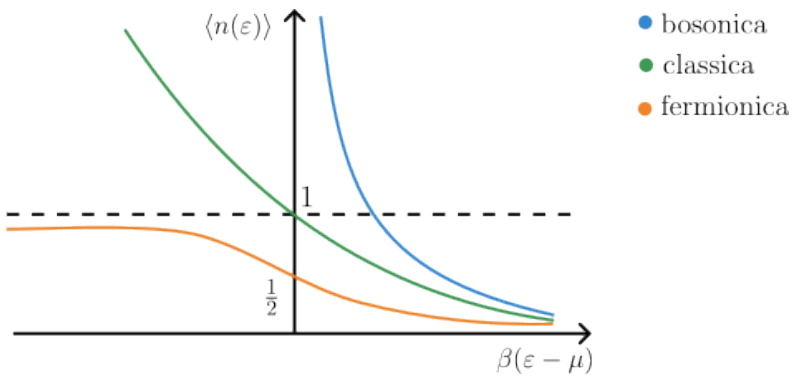
\includegraphics[width=0.6\linewidth]{Immagini/confronto statistiche.png}
    \caption{confronto tra le tre statistiche bosonica, fermionca e classica.}
    \label{fig: confronto statistiche}
\end{figure}

\subsubsection{Temperatura di Fermi}
Consistentemente al principio di esclusione, in ogni microstato fermionico si deve avere che $0 \le \vmedio{n(\epsilon)}_F \le 1$. Nel limite di bassa temperatura, $T \to 0$ e di conseguenza $\beta \to \infty$, per cui
\begin{equation}
    e^{\beta(\epsilon - \mu)} \simeq
    \begin{cases}
        0,\, \epsilon < \mu|_{T=0} \equiv \epsilon_F \\
        \infty,\, \epsilon > \epsilon_F
    \end{cases},
\end{equation}
dove il potenziale chimico del sistema $\epsilon_F$ a temperatura $T = 0$ prende il nome di `ènergia di Fermi'. Dall'espressione della statistica fermionica \eqref{eq: statistica Fermi-Dirac}, in questo limite si ha che
\begin{equation}
    \vmedio{n(\epsilon)}_F \simeq \Theta(\epsilon_ F - \epsilon).
\end{equation}
All'energia di fermi $\epsilon_F$ si può associare la ``temperatura di Fermi'' caratteristica del sistema come
\begin{equation}
    kT_F = \epsilon_F,
\end{equation}
la quale permette di intuire una scala di temperatura ed indicare i limiti di alta e bassa temperatura per un particolare sistema tramite la scala di energia. In altre parole, quando si parla di limite di bassa ed alta temperatura, si prende come punto di riferimento la temperatura $T_F$. Infatti, l'energia di Fermi risulta essere un parametro fondamentale per descrivere il comportamento di un sistema fermionico nel limite di bassa temperatura $T \ll T_F$. 

\subsubsection{Condensazione di Bose - Einstein}
Come detto, per ogni livello $\epsilon$ di un sistema bosonico si deve avere $\mu < \epsilon$; infatti, se così non fosse si avrebbe $\vmedio{n(\epsilon)}_B < 0$, ossia un risultato fisicamente privo di senso in quanto i numeri di occupazione assumono sempre valori maggiori o pari a zero. Quindi, dato che tale condizione sul potenziale chimico vale per ogni $\epsilon$, deve anche valere per il livello fondamentale $\epsilon_0$, per cui $\mu < \epsilon_0$ da cui, nel limite $\mu \to \epsilon_0^-$, segue che
\begin{equation}
\label{eq: condensazione Bose-Einstein}
    \lim_{\mu \to \epsilon_0^-}\vmedio{n(\epsilon)}_B = \infty.
\end{equation}
Normalmente, il numero di particelle che occupano i livelli è irrilevante rispetto ad infinito, tuttavia nel limite termodinamico il numero dei componenti tende proprio ad infinito; quindi una frazione macroscopica di componenti condensa nello stato fondamentale. Questo fenomeno prende il nome di ``condensazione di Bose - Einstein'' ed è prettamente di natura quantistica, ovvero non ha un analogo classico.

\section{Gas di fermioni liberi}
Si consideri un gas di particelle fermioniche libere occupanti un volume $V$ coincidente, per semplicità e senza perdere di generalità, con un cubo di lato $L$, assumendo inoltre che le condizioni al contorno delle funzioni d'onda siano periodiche. In tal caso, gli autostati dell'energia sono associati ai numeri quantici $\vn \in \Z^3$ e la loro energia è
\begin{equation}
    \epsilon(\vn) = \frac{\hbar^2}{2m}\bigg(\frac{2\pi}{L}\bigg)^2|\vn|^2 = \frac{\hbar^2}{2m}|\vk|^2.
\end{equation}
Se le particelle sono dotate di uno spin $s$, allora ogni autostato ha una degenerazione aggiuntiva $g_s = 2s + 1$, dovuta ai possibili autovalori $-\hbar s,\hbar(s - 1),\dots,\hbar(s - 1),\hbar s$ della terza componente di spin. Quindi, l'espressione del potenziale grancanonico è
\begin{equation}
\label{eq: potenziale gas di fermioni (grancanonico)}
    \varpi_F = -\frac{g_s}{\beta}\sum_{\vn\in\Z^3}\log{(1 + ze^{-\beta\epsilon(\vn)})}.
\end{equation}
Per calcolarlo, si deve seguire un certo procedimento. Prima di tutto, ci si concentra sul trovare l'espressione di $\varpi_F$ nel limite termodinamico, quindi si passa dal discreto al continuo con
\begin{equation}
\label{eq: passaggio al continuo gas di fermioni liberi}
    \sum_{\vn\in\Z^3}f(|\vn|) \longrightarrow \frac{V}{2\pi^2}\int_0^\infty dk\,k^2f(|\vk|).
\end{equation}
In questo caso, è più conveniente usare l'energia $\epsilon$ invece del modulo $|\vk| \equiv k$, perciò si opera il cambio di variabili
\begin{equation}
    \epsilon = \frac{\hbar^2}{2m}k^2\quad\Longrightarrow\quad dk = \frac{\sqrt{\pi}}{\lambda_T}\frac{\beta^{1/2}}{\epsilon^{{1/2}}}d\epsilon
\end{equation}
ottenendo
\begin{equation}
    \sum_{\vn\in\Z^3}f(|\vn|) \longrightarrow \frac{V}{V_T}\frac{2}{\sqrt{\pi}}\beta^{3/2}\int_0^\infty d\epsilon\,\epsilon^{1/2}f(\epsilon).
\end{equation}
Il potenziale grancanonico quindi diventa
\begin{equation}
    \begin{split}
        \varpi_F &= -\frac{g_s}{\beta}\frac{V}{V_T}\frac{2}{\sqrt{\pi}}\beta^{3/2}\int_0^\infty d\epsilon\,\epsilon^{1/2}\log(1 + ze^{-\beta\epsilon}) \\
        &= -\frac{g_s}{\beta}\frac{V}{V_T}\frac{2}{\sqrt{\pi}}\int_0^\infty dx\,x^{1/2}\log{(1 + ze^{-x})}
    \end{split},
\end{equation}
dove si è operato il cambio di variabili $x = \beta\epsilon$. L'integrale in questione può essere risolto in una forma standard integrando per parti ottenendo
\begin{equation}
    \frac{2}{\sqrt{\pi}}\int_0^\infty dx\,x^{1/2}\log{(1 + ze^{-x})} = \frac{1}{\Gamma(5/2)}\int_0^\infty dx\,\frac{x^{3/2}}{e^xz^{-1} + 1} \equiv f_{5/2}
\end{equation}
e di conseguenza
\begin{equation}
    \varpi_F = -\frac{g_s}{\beta}\frac{V}{V_T}f_{5/2}(z),
\end{equation}
dove si nota l'introduzione delle funzioni fermioniche $f_\nu(z)$ come
\begin{equation}
\label{eq: funzioni fermioniche}
    f_\nu(z) = \frac{1}{\Gamma(\nu)}\int_0^\infty dx\,\frac{x^{\nu - 1}}{e^xz^{-1} + 1}.
\end{equation}
\begin{obs}
    Le funzioni fermioniche definite nella \eqref{eq: funzioni fermioniche} godono della proprietà di ricorrenza 
    \begin{equation}
        z\frac{\p f_\nu}{\p z} = f_{\nu -1}.
    \end{equation}
    Questa può essere dimostrata partendo da 
    \begin{equation}
        z\frac{\p f}{\p z} = \frac{1}{\Gamma(\nu)}\int_0^\infty dx\,x^{\nu -1}z\frac{\p}{\p z}\bigg(\frac{1}{e^xz^{-1} + 1}\bigg)
    \end{equation}
    e notando che per qualsiasi funzione $F$ si ha
    \begin{equation}
        z\frac{\p}{\p z}F(e^xz^{-1}) = -\frac{\p}{\p x}F(e^xz^{-1});
    \end{equation}
    pertanto, integrando per parti si ha, si ha
    \begin{equation}
        \begin{split}
            z\frac{\p f}{\p z} = -\frac{1}{\Gamma(\nu)}\int_0^\infty dx\,x^{\nu -1}\frac{\p}{\p x}\bigg(\frac{1}{e^xz^{-1} + 1}\bigg) &= \frac{\nu - 1}{\Gamma(\nu)}\int_0^\infty dx\,\frac{x^{\nu - 2}}{e^xz^{-1} + 1} \\
            &= \frac{1}{\Gamma(\nu - 1)}\int_0^\infty dx\, \frac{x^{(\nu - 1) - 1}}{e^xz^{-1} + 1} \\
            &\equiv f_{\nu - 1}(z).
        \end{split} 
    \end{equation}
    Inoltre, sono funzioni perfettamente regolari, monotone crescenti e che si annullano, per definizione, in $z = 0$ per ogni valore di $\nu$.
\end{obs}
Noto il potenziale $\varpi_F$ è adesso possibile derivare la termodinamica del sistema. La pressione $p$ e la densità $1/v$ sono date da
\begin{align}
\label{eq: pressione e densità gas fermioni liberi (grancanonico)}
    p &= -\frac{\varpi_F}{V} = g_s\frac{kT}{V_T}f_{5/2}(z), \\
    \frac{1}{v} &= \frac{\vmedio{N}_F}{V} = -\frac{\beta}{V}z\frac{\p\varpi_F}{\p z}\bigg|_{T,V} = \frac{g_s}{V_T}\frac{\p f_{5/2}(z)}{\p z} = \frac{g_s}{V_T}f_{3/2}(z).
\end{align}
Invece, l'energia interna è data da
\begin{equation}
    \begin{split}
        \vmedio{E} = \frac{\p}{\p\beta}(\beta\varpi_F)\bigg|_{V,z} &= -g_s\frac{\p}{\p\beta}\bigg(\frac{V}{V_T}f_{5/2}(z)\bigg) \\
        &= -g_sVf_{5/2}(z)\frac{\p}{\p\beta}\bigg(\frac{1}{V_T}\bigg) \\
        &= \frac{3}{2}Vg_s\frac{kT}{V_T}f_{5/2}(z) \\
        &=\frac{3}{2}pV,
    \end{split}
\end{equation}
dove si usato il fatto che
\begin{equation}
    \frac{1}{V_T} = \frac{1}{\lambda_T^3} \propto \beta^{-3/2}\quad\Longrightarrow\quad \frac{\p}{\p\beta}\bigg(\frac{1}{V_T}\bigg) = -\frac{3}{2}\frac{1}{\beta V_T}.
\end{equation}
Può essere utile, in particolare per il confronto con i dati sperimentali, considerare come variabile di controllo la densità $1/v$ invece che il potenziale chimico o la fugacità. Infatti, nel caso di un gas nella pratica è molto più semplice controllare la sua densità che gli altri due parametri. Questo tuttavia implica tornare all'ensemble canonico, dove appunto l'insieme delle variabili di controllo sono $\{T,V,1/v\}$ o, equivalentemente, $\{T,V,N\}$. Questo cambio di insieme di variabili può essere effettuato semplicemente invertendo la rispettiva equazione in \eqref{eq: pressione e densità gas fermioni liberi (grancanonico)} e definendo il parametro $\xi$ di proporzionalità alla densità come
\begin{equation}
\label{eq: parametro fermionico}
    \xi = \frac{V_T}{g_sv};
\end{equation}
questo parametro rappresenta il numero di componenti medio in un volume termico $V_T = \lambda_T^3$ e lega il limite classico per cui $z \to 0$ al limite di bassa densità o di alta temperatura dove $\xi \to 0$ tramite la relazione
\begin{equation}
    \xi = f_{3/2}(z).
\end{equation}
Dato che le funzioni fermioniche sono monotone, quest'ultima relazione può essere invertita in termini della fugacità per qualsiasi limite ottenendo
\begin{equation}
    z(\xi) = f_{3/2}^{-1}(\xi).
\end{equation}
Quindi adesso per esprimere le grandezze termodinamiche in funzione di $\xi$ si deve operare la sostituzione $z \to f^{-1}_\nu(\xi)$, in questo modo le espressioni della pressione $p$, della densità $1/v$ e dell'energia interna $\vmedio{E}$ diventano
\begin{align}
    p &= \frac{kT}{v\xi}f_{5/2}(f_{3/2}^{-1}(\xi)), \\ 
    \frac{1}{v} &= \frac{g_s}{V_T}f_{3/2}(f_{3/2}^{-1}(\xi)), \\
    E &= \frac{3}{2}NkT\frac{1}{\xi}f_{5/2}(f_{3/2}^{-1}(\xi)).
\end{align}
Anche se queste relazioni sono valide per ogni valore di $\xi$, ci si concentra sulla loro espansione nei due regimi di alta e bassa temperatura. Inoltre, l'equazione di stato meccanica è
\begin{equation}
\label{eq: equazione di stato meccanica gas fermioni liberi}
    pV = \vmedio{N}kT\frac{1}{\xi}f_{5/2}(f_{3/2}^{-1}(\xi)).
\end{equation}

\setcounter{caso}{0}
\begin{caso}[alta temperatura]
    Le funzioni fermioniche per definizione, data da \eqref{eq: funzioni fermioniche}, ammettono per $z \to 0$ la seguente espansione in serie\footnote{L'espansione si ottiene dalla con un'espansione geometrica dell'integrando 
    \begin{equation}
        \begin{split}
            f_\nu(z) = \frac{1}{\Gamma(\nu)}\int_0^\infty dx\,x^{\nu -1} \frac{ze^{-x}}{1 + ze^{-x}} &= \frac{1}{\Gamma(\nu)}\int_0^\infty dx\,x^{\nu -1}ze^{-x}\sum_{n=0}^\infty(-ze^{-x})^n \\
            &= \frac{1}{\Gamma(\nu)}\sum_{l=1}^\infty(-1)^{l-1}z^l\int_0^\infty dx\,x^{\nu-1}e^{-lx} \\
            &\overset{w = lx}{=} \cancel{\frac{1}{\Gamma(\nu)} }\sum_{l=1}^\infty(-1)^{l-1}\frac{z^l}{l^\nu}\cancel{\int_0^\infty dw\,w^{\nu - 2}e^{-w}}.
        \end{split}
    \end{equation}
    }
    \begin{equation}
    \label{eq: espansione f alta T}
        f_\nu(z) = \sum_{l = 1}^\infty(-1)^{l-1}\frac{z^l}{l^\nu} = z - \frac{z^2}{2^\nu} + \frac{z^3}{3^\nu} + \cdots.
    \end{equation}
    Quindi, sapendo che $z \to 0$ implica $\xi \to 0$ l'espansione in serie della funzione inversa deve essere
    \begin{equation}
    \label{eq: espazione z alta T}
        z(\xi) = f_\nu^{-1}(\xi) = \alpha_1 \xi + \alpha_2\xi^2 + \alpha_3 \xi^3 + \cdots,
    \end{equation}
    per cui se si applica la \eqref{eq: espazione z alta T} nella \eqref{eq: espansione f alta T}, nel caso in cui $\nu = 3/2$, si ha
    \begin{equation}
        \alpha_1 \xi + \alpha_2\xi^2  + \cdots - \frac{1}{2^\nu}(\alpha_1\xi + \alpha_2\xi^2 + \cdots)^2 + \frac{1}{3^\nu}(\alpha_1\xi + \alpha_2\xi^2 + \cdots)^3 + \cdots = \xi.
    \end{equation}
    Uguagliando adesso i coefficienti dello stesso grado in $\xi$ si ottengono i valori dei coefficienti $\alpha_i$
    \begin{align}
        \alpha_1\xi = \xi\quad&\Longrightarrow\quad \alpha_1 = 1, \\
        \alpha_2\xi^2 - \frac{\alpha_1^2\xi^2}{2^\nu} = 0\quad&\Longrightarrow\quad \alpha_2 = \frac{1}{2^\nu}, \\
        \alpha_3 - \frac{2}{(2^\nu)^2} + \frac{1}{3^\nu} = 0\quad&\Longrightarrow\quad \alpha_3 = \frac{1}{2^{\nu-1}} - \frac{1}{3^\nu}\dots
    \end{align}
    Quindi, sostituendo i coefficienti $\alpha_i$ nella \eqref{eq: espazione z alta T}, si ha
    \begin{equation}
        z(\xi) = f_{3/2}^{-1}(\xi) = \xi + \frac{\xi^2}{2^{3/2}} + \bigg(\frac{1}{4} - \frac{1}{3^{3/2}}\bigg)\xi^3 + \cdots
    \end{equation}
    e, di conseguenza, l'equazione di stato \eqref{eq: equazione di stato meccanica gas fermioni liberi} diventa
    \begin{equation}
    \label{eq: equazione di stato meccanica gas fermioni liberi (espansione in serie)}
        \begin{split}
            pV = \vmedio{N}kT\frac{1}{\xi}\sum_{l=1}^\infty(-1)^{l-1}\frac{z^l}{l^{5/2}} &= \vmedio{N}kT\frac{1}{\xi}\bigg[\xi + \xi^2 \bigg(\frac{1}{2^{3/2}} - \frac{1}{2^{5/2}}\bigg) + \cdots\bigg] \\
            &= NkT\bigg(1+ \frac{\xi}{2^{5/2}} + \cdots\bigg).
        \end{split}
    \end{equation}
    Dunque, l'introduzione della statistica fermionica ha causato una correzione nell'equazione di stato meccanica classica, in particolare alla densità, le quali sono analoghe a quelle ottenute per i gas interagenti aventi un potenziale di interazione a corto raggio. La serie in cui si presenta l'equazione \eqref{eq: equazione di stato meccanica gas fermioni liberi (espansione in serie)} è ben nota e prende il nome di ``espansione viriale'', in generale si può esprimere in una forma più compatta introducendo i coefficienti di espansione viriale $b_i$ così da avere
    \begin{equation}
        pV = \vmedio{N}kT\sum_{l=1}^\infty b_l\xi^{l-1}.
    \end{equation}
\end{caso}

\begin{caso}[bassa temperatura]
    Se il limite $z \to 0$ corrisponde al limite classico, il limite $z \to \infty$ corrisponde a quello quantistico. Chiaramente, per definizione $z \to \infty$ implica $\xi \to \infty$, quindi si deve ora studiare l'espansione asintotica delle funzioni fermioniche $f_\nu(z)$. Per farlo, si riscrive la forma generica delle $f_\nu(z)$ come
    \begin{equation}
        f_\nu(z) = \frac{1}{\Gamma(\nu)}\int_0^\infty dx\,\frac{x^{\nu - 1}}{e^{x - \xi} + 1},\quad z = e^\xi.
    \end{equation}
    A questo punto è conveniente spezzare l'integrale sui due intervalli $[0,\xi]$ e $[\xi,\infty)$, in modo da avere
    \begin{equation}
        \begin{split}
            f_\nu(z) &= \frac{1}{\Gamma(\nu)} \bigg( \int_{0}^{\xi}dx\, \frac{x^{\nu-1}}{e^{x-\xi}+1} + \int_{\xi}^{\infty}dx\, \frac{x^{\nu-1}}{e^{x-\xi}+1} \bigg) \\
            &= \frac{1}{\Gamma(\nu)} \bigg( \int_{0}^{\xi}dx\,x^{\nu-1}\frac{e^{\xi-x}}{1+e^{\xi-x}} + \int_{\xi}^{\infty}dx\, \frac{x^{\nu-1}}{e^{x-\xi}+1} \bigg) \\ 
            &= \frac{1}{\Gamma(\nu)} \bigg( \frac{\xi^{\nu}}{\nu} - \int_{0}^{\xi}dx\,  \frac{x^{\nu-1}}{e^{\xi-x}+1} + \int_{\xi}^{\infty}dx\,  \frac{x^{\nu-1}}{e^{x-\xi}+1}\bigg),
        \end{split}
    \end{equation}
    dove, per il primo integrale, nel secondo passaggio si è moltiplicato per $e^{x-\xi}$, nel terzo passaggio si è raccolto $x^{\nu-1}$ e nell'ultimo passaggio si è svolto il primo termine $\int_0^\xi dx\,x^{\nu - 1} = \xi^\nu/\nu$. Ci si aspetta che dopo il primo termine dominante appaiano delle correzioni sempre più trascurabili per $\xi \to \infty$. Ora si opera un cambio di variabili $\eta = \xi - x$ nel primo integrale, mentre nel secondo si pone $\eta = x - \xi$, ottenendo
    \begin{equation}
        \begin{split}
            f_\nu(z) &= \frac{1}{\Gamma(\nu)} \bigg( \frac{\xi^{\nu}}{\nu} - \int_{\xi}^{0}d\eta\,  (-1)\frac{(\xi - \eta)^{\nu-1}}{e^\eta+1} + \int_{\xi}^{\infty}d\eta\,  \frac{(\xi + \eta)^{\nu-1}}{e^{\eta}+1}\bigg) \\
            &= \frac{1}{\Gamma(\nu)} \bigg( \frac{\xi^{\nu}}{\nu} - \int_{0}^{\xi}d\eta\, \frac{(\xi - \eta)^{\nu-1}}{e^\eta+1} + \int_{\xi}^{\infty}d\eta\,  \frac{(\xi + \eta)^{\nu-1}}{e^{\eta}+1}\bigg).
        \end{split} 
    \end{equation}
    Se $\xi \ge 1$, allora $(e^\eta + 1)^{-1} \to 0$ e i contributi di ordine maggiore in $\xi$ sono sempre più trascurabili, quindi integrare su $[0,\xi]$ o su $[0,\infty)$ è indifferente. Con questa considerazione si può quindi scrivere
    \begin{equation}
        \begin{split}
            f_\nu(z) &\simeq \frac{1}{\Gamma(\nu)} \bigg( \frac{\xi^{\nu}}{\nu} - \int_{0}^{\infty}d\eta\, \frac{(\xi - \eta)^{\nu-1}}{e^\eta+1} + \int_{\xi}^{\infty}d\eta\,  \frac{(\xi + \eta)^{\nu-1}}{e^{\eta}+1}\bigg) \\
            &= \frac{1}{\Gamma(\nu)} \bigg\{ \frac{\xi^{\nu}}{\nu} + \int_{0}^{\infty}\frac{d\eta}{e^\eta+1}\bigg[ (\xi + \eta)^{\nu-1} - (\xi - \eta)^{\nu-1} \bigg]\bigg\} \\
            &= \frac{1}{\Gamma(\nu)} \bigg\{ \frac{\xi^{\nu}}{\nu} + \int_{0}^{\infty}\frac{d\eta}{e^\eta+1}\bigg[\sum_{k=0}^\infty\binom{\nu - 1}{k}\eta^k\xi^{\nu - 1 -k} \\
            &- \sum_{k=0}^\infty\binom{\nu-1}{k}(-1)^k\eta^k\xi^{\nu - 1 - k} \bigg]\bigg\} \\
            &= \frac{1}{\Gamma(\nu)} \bigg(\frac{\xi^\nu}{\nu} + \int_0^\infty\frac{d\eta}{e^\eta  + 1}2\sum_{k_{odd}}\binom{\nu - 1}{k}\eta^k\xi^{\nu - 1 -k}\bigg),
        \end{split}
    \end{equation}
    dove nel secondo passaggio si è usata l'espansione binomiale\footnote{La forma generale dell'espansione binomiale è $(a + b)^n = \nsum_{k=0}^n\binom{n}{k}a^{n-k}b^k$.} e nel terzo  si è scritto tutto con un'unica somma sui valori dispari di $k$ dato che il termine $(-1)^k$ comporta la cancellazione dei termini pari e la somma di quelli dispari, da qui anche il fattore due davanti a tale somma. Ora l'obiettivo è quello di calcolare l'integrale su $\eta$ che compare nell'espressione di $f_\nu(z)$, quindi
    \begin{equation}
        \begin{split}
            I_k \equiv \int_0^\infty\frac{d\eta}{e^\eta  + 1}\eta^k = \int_0^\infty d\eta\,\eta^k\frac{e^{-\eta}}{1 + e^{-\eta}} &= \int_0^\infty d\eta\,\eta^ke^{-\eta}\sum_{p=0}^\infty (-1)^pe^{-p\eta} \\
            &= \sum_{q=1}^\infty (-1)^{q-1}\int_0^\infty d\eta\,\eta^ke^{-q\eta} \\
            &\overset{t = q\eta}{=}\sum_{q=1}^\infty \frac{(-1)^{q-1}}{q^{k+1}} \int_0^\infty dt\,t^ke^{-t} \\
            &= \Gamma(k+1)\sum_{q=1}^\infty \frac{(-1)^{q-1}}{q^{k+1}}.
        \end{split}
    \end{equation}
    La somma sull'indice $q$ in $I_k$ può essere ulteriormente divisa nelle due somme sui valori pari e dispari di $q$ così da ottenere
    \begin{equation}
        \begin{split}
            I_k &= \Gamma(k+1)\bigg(\sum_{q_{odd}}\frac{1}{q^{k+1}} - \sum_{q_{even}}\frac{1}{q^{k+1}}\bigg) \\
            &= \Gamma(k +1)[\xi_{odd}(k+1) - \xi_{even}(k+1)].
        \end{split}
    \end{equation}
    Adesso si nota che se si avesse $\xi_{odd}(k+1) + \xi_{even}(k+1)$ questa somma corrisponderebbe alla Zeta di Riemann $\zeta$. Tuttavia, in questo caso si ha una differenza, per cui ci si chiede come si possa ricondurre questa alla Zeta di Riemann. Prima di tutto, si ricorda che esiste una relazione tra le $\xi$ e la $\zeta$ date da
    \begin{align}
        \xi_{even}(k+1) &\overset{q = 2n}{=} \sum_{n = 1}^\infty\frac{1}{(2n)^{k+1}} = \frac{1}{2^{k+1}}\sum_{n=1}^\infty\frac{1}{n^{k+1}} = \frac{1}{2^{k+1}}\zeta(k+1), \\
        \xi_{odd}(k+1) &= \zeta(k+1) - \xi_{even}(k+1) = \bigg(1 - \frac{1}{2^{k+1}}\bigg)\zeta(k+1).
    \end{align}
    Quindi, immediatamente si ha che
    \begin{equation}
        \begin{split}
            \xi_{odd}(k+1) - \xi_{even}(k+1) &= \bigg(1 - \frac{1}{2^{k+1}}\bigg)\zeta(k+1) - \frac{1}{2^{k+1}}\zeta(k+1) \\
            &= \zeta(k+1)\bigg(1 - \frac{1}{2^k}\bigg).
        \end{split}
    \end{equation}
    Pertanto, finalmente si trova che l'integrale vale
    \begin{equation}
        I_k = \Gamma(k+1)\zeta(k+1)\bigg(1 - \frac{1}{2^k}\bigg).
    \end{equation}
    Ritornando allora all'espressione di $f_\nu(z)$ sostituendo il risultato appena ottenuto per $I_k$ si arriva a 
    \begin{equation}
        \begin{split}
            f_\nu(z) & \simeq \frac{(\ln{z})^\nu}{\Gamma(\nu + 1)}\bigg[1 + 2\nu\sum_{k_{odd}}\binom{\nu-1}{k}\Gamma(k+1)\zeta(k+1)\bigg(1 - \frac{1}{2^k}\bigg)\frac{1}{(\ln{z})^{k+1}}\bigg] \\
            &= \frac{(\ln{z})^\nu}{\Gamma(\nu + 1)}\bigg[1 + \frac{\pi^2}{6}\nu(\nu - 1)(\ln{z})^{-2} + \cdots\bigg].
        \end{split}
    \end{equation}
    Dunque, si è trovata una prima approssimazione delle funzioni $f_\nu(z)$ come 
    \begin{equation}
        f_\nu(z) \simeq \frac{(\ln{z})^\nu}{\Gamma(\nu + 1)}.
    \end{equation}
    Ora, questo risultato si può usare per scrivere $\xi$ in funzione del potenziale chimico $\mu$ ricordando che $z = e^{\beta\mu}$, per cui 
    \begin{equation}
        \xi = f_{3/2}(z) \simeq  \frac{(\beta\mu)^{3/2}}{\Gamma(5/2)}\bigg[1 + \frac{\pi}{8}(\beta\mu)^{-2} + \cdots \bigg].
    \end{equation}
    Al primo ordine, si ottiene il risultato completo per il limite $T \to 0$ dato da
    \begin{equation}
        \Gamma(5/2)\xi  =(\beta\mu|_{T=0})^{3/2} \equiv (\beta\epsilon_F)^{3/2},
    \end{equation}
    l'energia di Fermi così definita tramite il potenziale chimico è direttamente legato alla densità del sistema
    \begin{equation}
        \epsilon_F = \frac{\hbar^2}{2m}\bigg(\frac{3}{4\pi g_sv}\bigg)^{3/2},\quad \xi = \frac{V_T}{g_sv}.
    \end{equation}
    Al secondo ordine invece si ha
    \begin{equation}
        (\beta\epsilon_F)^{3/2} \simeq (\beta\mu)^{3/2}\bigg[1 + \frac{\pi^2}{8}(\beta\mu)^{-2}\bigg]
    \end{equation}
    che, imponendo l'ansatz $\beta\mu = \beta\epsilon_F[1 + \alpha(\beta\epsilon_F)^{-2} + \cdots]$, diventa
    \begin{equation}
        \begin{split}
            (\beta\epsilon_F)^{3/2}  &= (\beta\epsilon_F)^{3/2} [1 + \alpha(\beta\epsilon_F)^{-2} + \cdots]^{3/2} \\
            &\times\bigg\{1 + \frac{\pi^2}{8}(\beta\epsilon_F)^{-2}[1 + \alpha(\beta\epsilon_F)^{-2} + \cdots]^{-2}\bigg\} \\
           1 &\simeq \bigg[1 + \frac{3}{2}\alpha(\beta\epsilon_F)^{-2}\bigg] \bigg[1 + \frac{\pi^2}{8}(\beta\epsilon_F)^{-2}\bigg] \\
           1 &\simeq 1 + \bigg(\frac{3}{2}\alpha + \frac{\pi^2}{8}\bigg)(\beta\epsilon_F)^{-2},
        \end{split}
    \end{equation}
    da cui si trova immediatamente che 
    \begin{equation}
        \alpha = -\frac{\pi^2}{12}.
    \end{equation}
    Dunque, è possibile passare all'ensemble canonico tramite
    \begin{equation}
        \beta\mu = \beta\epsilon_F\bigg[1 - \frac{\pi^2}{12}(\beta\epsilon_F)^{-2} + \cdots\bigg],\quad \beta\epsilon_F = [\Gamma(5/2)\xi]^{2/3}.
    \end{equation}
    Nel limite quantistico, l'equazione di stato meccanica \eqref{eq: equazione di stato meccanica gas fermioni liberi (espansione in serie)} assume adesso la forma
    \begin{equation}
        \begin{split}
            pV &= \vmedio{N} k T \frac{\Gamma(5/2)}{(\beta \epsilon_F)^{3/2}} \frac{(\beta \epsilon_F)^{5/2}}{\Gamma(7/2)} \bigg[ 1 - \frac{\pi^2}{12}(\beta \epsilon_F)^{-2} + \cdots \bigg]^{5/2} \\
            &\times\bigg[ 1 + \frac{5}{8}\pi^2 (\beta \epsilon_F)^{-2}(1+\cdots) \bigg] \\
            &= \frac{2}{5} \vmedio{N} \epsilon_F
            \bigg[ 1 + \frac{5\pi^2}{12}(\beta \epsilon_F)^{-2} + \cdots \bigg] \\ 
            &= \frac{2}{5} \vmedio{N} \epsilon_F \bigg[ 1 + \frac{5\pi^2}{12}\bigg(\frac{T}{T_F}\bigg)^2 + \cdots \bigg],
            \end{split} 
    \end{equation}
    mentre per l'energia interna si ha
    \begin{equation}
        \vmedio{E} = \frac{3}{2} pV = \frac{3}{5} \vmedio{N} \epsilon_F
        \bigg[ 1 + \frac{5\pi^2}{12}\bigg(\frac{T}{T_F}\bigg)^2 + \cdots \bigg].
    \end{equation}
    Anche a $T = 0$ (in cui conta solo il primo termine di queste espansioni), si ha una pressione $p_F$ non nulla, che prende il nome di ``pressione di Fermi''
    \begin{equation}
        p_FV = \frac{2}{5} \vmedio{N} \epsilon_F,
    \end{equation}
    con la quale si può esprimere l'energia media a temperatura nulla
    \begin{equation}
        \vmedio{E}_F = \frac{3}{5} \vmedio{N} \epsilon_F.
    \end{equation}
    Quindi in generale, per un gas di fermioni si trova che a temperatura nulla, la pressione e l'energia non sono anch'esse nulle; ciò è dovuto al fatto che anche per $T = 0$ tutti fermioni non si possono disporre sul livello più basso, per via del principio di esclusione di Pauli. Infatti, come visto a $T = 0$ il numero medio di occupazione $\vmedio{n(\epsilon)}_p$ è una funzione Theta di Heaviside. Tutti i livelli fino all'energia di Fermi devono essere occupati, mentre da lì poi nessun livello deve essere occupato. Quindi anche a temperatura nulla, sono comunque occupati degli stati eccitati. Pertanto, utilizzando la \eqref{eq: passaggio al continuo gas di fermioni liberi} per esprimere la degenerazione dei livelli energetici si ottiene esattamente la relazione precedente
    \begin{equation}
        \vmedio{E} = \frac{g_sV}{V_T}\frac{2}{\sqrt{\pi}}\beta^{3/2}\int_0^\infty d\epsilon\,\epsilon^{1/2}\Theta(\epsilon_F - \epsilon).
    \end{equation}
    Per quanto riguarda la capacità termica, nel limite quantistico si ha 
    \begin{equation}
        c_{V,N} = \frac{\p\vmedio{E}}{\p T}\bigg|_{V,N} = \frac{3}{5}N\epsilon_F\bigg[\frac{5}{12}\pi^2\frac{2T}{T_F^2} + \cdots\bigg],
    \end{equation}
    che tende a zero linearmente in accordo con il teorema di Nernst. In generale, l'andamento della capacità termica è perfettamente regolare, come si vede in figura \ref{fig: andamento cap. termica (gas fermioni liberi)}. 
\end{caso} 
\begin{figure}[h]
    \centering
    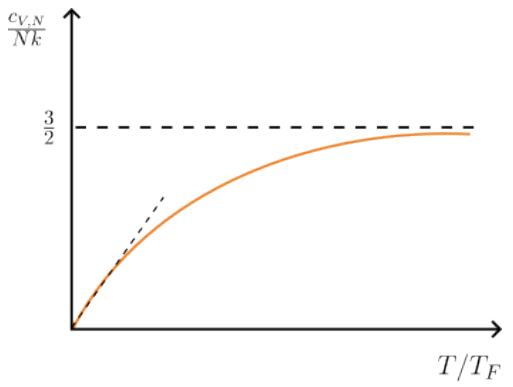
\includegraphics[width=0.5\linewidth]{Immagini/andamento cap. termica (gas fermioni liberi).png}
    \caption{andamento di $c_{V,N}/kN$ in funzione di $T/T_F$ per un gas di fermioni liberi.}
    \label{fig: andamento cap. termica (gas fermioni liberi)}
\end{figure}
\subsection{Elettroni liberi nei metalli}
Nei metalli, gli elettroni di conduzione hanno un'elevata mobilità e la loro termodinamica viene ben riprodotta approssimandoli ad un gas di fermioni liberi di spin $s = 1/2$, cioè $g_s = 2s + 1 = 2$ e quindi con energia di Fermi pari a 
\begin{equation}
    \epsilon_F = \frac{h^2}{2m}\bigg(\frac{3}{8\pi} - \frac{1}{v}\bigg)^{2/3}.
\end{equation}
Si può stimare la densità in funzione del numero di elettroni presenti nel reticolo cristallino come
\begin{equation}
    \frac{1}{v} = \frac{f_ef_a}{a^3},
\end{equation}
dove $f_e$ ed $f_a$ sono rispettivamente il numero di elettroni di conduzione per atomo e quello di atomi per cella del reticolo. Essenzialmente, si contano quanti elettroni di conduzione ci sono per ogni cella e si divide tale numero per il volume della singola cella. Ad esempio, nel caso del sodio l'energia di fermi è
\begin{equation}
    \epsilon_F(\mathrm{Na}) \simeq \SI{5.03e-13}{\joule},
\end{equation}
a cui corrisponde la temperatura di Fermi
\begin{equation}
    T_F(\mathrm{Na}) \simeq \SI{3.64e4}{\kelvin}.
\end{equation}
Dunque, a temperatura ordinaria gli elettroni di conduzione nei metalli formano un gas in un regime profondamente quantistico.

\section{Gas di bosoni liberi}
Per semplicità, si considera un sistema di bosoni aventi spin nullo così che si possa porre $g_s = 0$ semplificando i calcoli; comunque, non è complesso estendere il risultato al caso generale con $g_s = 2s + 1$ dove $s$ è un intero. Ad ogni modo, il procedimento per il gas di bosoni è del tutto analogo a quanto fatto nel caso fermionico. In questo caso, il potenziale grancanonico, invece che \eqref{eq: potenziale gas di fermioni (grancanonico)}, è
\begin{equation}
    \varpi_B = \frac{1}{\beta}\sum_{\vn\in\Z^3}\log{\bigg(1 - ze^{-\beta\epsilon(\vn)}\bigg)}.
\end{equation}
Anche adesso si potrebbe passare dal discreto al continuo tramite un integrale su $\epsilon$ nel limite termodinamico. Tuttavia, facendo l'integrale si sta assegnando ad ogni livello $\epsilon$ una misura nulla, incluso il livello fondamentale $\epsilon_0$. Quest'ultimo però nel caso bosonico assume un ruolo particolare: in questo può condensare una frazione macroscopica di componenti per $\mu \to 0^-$ come discusso nella \eqref{eq: condensazione Bose-Einstein}. Pertanto, non è corretto in generale assegnare misura nulla al contributo di $\epsilon_0$. Si separa quindi quest'ultimo da tutti gli altri associati agli stati eccitati prima di sostituire la somma discreta con l'integrale
\begin{equation}
    \varpi_B = \frac{1}{\beta}\bigg[\log{(1-z)} + \frac{V}{V_T}\frac{2}{\sqrt{\pi}}\beta^{3/2}\int_0^\infty d\epsilon\,\epsilon^{1/2}\log{(1-ze^{-\beta\epsilon})}\bigg].
\end{equation}
Adesso, operando il cambio di variabili $x = \beta\epsilon$ e integrando per parti l'integrale
\begin{equation}
    \frac{2}{\sqrt{\pi}}\int_0^\infty d\epsilon\,(\beta\epsilon)^{1/2}\log{(1-ze^{-\beta\epsilon})} = \frac{-1}{\Gamma(5/2)}\int_0^\infty dx\,\frac{x^{3/2}}{e^xz^{-1} - 1} \equiv -g_{5/2}(z),
\end{equation}
il potenziale $\varpi_B$ diventa
\begin{equation}
    \varpi_B = \frac{1}{\beta}\bigg[\log{(1-z)} - \frac{V}{V_T}g_{5/2}(z)\bigg],
\end{equation}
dove si nota l'introduzione delle funzioni bosoniche $g_\nu(z)$ come
\begin{equation}
    g_\nu(z) = \frac{1}{\Gamma(\nu)}\int_0^\infty dx\,\frac{x^{\nu-1}}{e^xz^{-1} - 1}.
\end{equation}
\begin{obs}
    Anche per le funzioni bosoniche vale una relazione di ricorrenza del tipo
    \begin{equation}
        z\frac{\p g_\nu}{\p z} = g_{\nu - 1}.
    \end{equation}
    Inoltre, sono tutte ben definite, regolari e monotone crescenti, ma solamente nell'intervallo $z \in [0,1]$, a parte la funzione $g_{1/2}(z)$ che risulta asintoticamente divergente ad infinito in $z = 1$ .
\end{obs}
Nelll'intervallo $z\in[0,1]$ le funzioni bosoniche ammettono la rappresentazione in serie 
\begin{equation}
\label{eq: funzioni bosonoiche (espansione in serie)}
    g_\nu(z) = \sum_{l=1}^\infty\frac{z^l}{l^\nu} = z + \frac{z^2}{2^\nu} + \frac{z^3}{3^\nu}+ \cdots,
\end{equation}
in particolare il valore massimo di di queste queste funzioni è 
\begin{equation}
    g_\nu(1) = \sum_{l=1}^\infty\frac{1}{l^\nu} \equiv \zeta(\nu).
\end{equation}
Noto il potenziale, la termodinamica segue come immediatamente
\begin{align}
\label{eq: pressione e densità gas bosoni liberi (grancanonico)}
    p &= -\frac{\varpi_B}{V} = kT\bigg[-\frac{\log{(1-z)}}{V} + \frac{g_{5/2}(z)}{V_T}\bigg], \\
    \frac{1}{v} &= -\frac{\beta z}{V}\frac{\p\varpi_B}{\p z}\bigg|_{T,V} = \frac{1}{V}\bigg[\frac{z}{1-z} + \frac{V}{V_T}g_{3/2}(z)\bigg], 
\end{align}
dove per la densità il primo termine corrisponde al numero medio di particelle nello stato fondamentale $N_0 = z/(1-z)$, mentre il secondo corrisponde al numero medio di particelle in tutti gli stati eccitati $N_e = \vmedio{N} - N_0$. Dalla definizione di $N_0$, si nota che per $z \to 1$ questo diverge ad infinito, ma può crescere al più come $N$ nel limite termodinamico, in quanto non ci possono essere più particelle nello stato fondamentale di quelle totali. Quindi, il primo termine della pressione nella \eqref{eq: pressione e densità gas bosoni liberi (grancanonico)} viene soppresso nel limite termodinamico dato che
\begin{equation}
    -\frac{kT}{V}\log{(1-z)} \simeq \frac{kT}{V}\log{(N_0 + 1)} \le \frac{kT}{V}\log{(N + 1)} \simeq \frac{\log{N}}{N},
\end{equation}
per cui $p$ e $1/v$ nel limite termodinamico diventano
\begin{equation}
    p \simeq \frac{kT}{V_T}g_{5/2}(z),\quad \frac{1}{v} \simeq \frac{1}{V}(N_0 + N_e).
\end{equation}
Invece, per quanto riguarda l'energia interna $\vmedio{E}$, la derivazione nel caso bosonico è identica a quella di quella fermionico e pertanto restituisce 
\begin{equation}
    \vmedio{E} = \frac{3}{2}pV.
\end{equation}
Dunque, essendo le funzioni bosoniche superiormente limitate, a $T$ e $V$ fissati esiste un numero massimo di componenti che possono occupare gli stati eccitati dato da
\begin{equation}
    N_e \le \frac{V}{V_T}\zeta(3/2) \equiv \hatN.
\end{equation}
Assumendo il punto di vista canonico, ossia considerando la densità come variabile indipendente e la fugacità $z$ come dipendente, il sistema assume un comportamento diverso quando $N$ è inferiore o superiore al valore critico $\hatN$. Questa condizione critica può anche essere espressa in termini della densità o, analogamente, del parametro $\eta$ di proporzionalità alla densità come
\begin{equation}
\label{eq: parametro bosonico}
    \eta \equiv \frac{V_T}{v};
\end{equation}
questo parametro è il corrispettivo del parametro $\xi$ definito nella \eqref{eq: parametro fermionico}. Quindi, si passa dal valore critico $\hatN$ a $\hateta$ definito come
\begin{equation}
    \hateta \equiv \zeta(3/2);
\end{equation}
questo parametro critico implica che quando si raggiunge il numero di 2.61 particelle per volume termico a disposizione non è possibile aggiungerne altre, che quindi possono solo occupare lo stato fondamentale. Questa condizione, a $N$ e $V$ fissati, individua la temperatura critica $\hatT$ data da
\begin{equation}
\label{eq: temperatura critica gas di bosoni (grancanonico)}
    \hatT = \frac{h^2}{2\pi mk}[v\zeta(3/2)]^{-2/3},
\end{equation}
dove si è passato dalla relazione
\begin{equation}
    V_{\hatT} = v\zeta(3/2),\quad V_{\hatT} = \lambda_{\hatT}^{3} = \bigg(\frac{h^2}{2\pi mkT}\bigg)^{3/2}.
\end{equation}
A questo punto, è possibile distinguere i soliti due limiti di alta e bassa temperatura, detti rispettivamente regime ``usuale'' e ``di condensazione''. 

\setcounter{caso}{0}
\begin{caso}[alta temperatura]
    Nel regime usuale, ossia nel limite di alta temperatura, il parametro $\eta$ soddisfa la relazione $\eta < \zeta(3/2)$ e consistentemente $z < 1$. Questa condizione si può vedere in due modi:
    \begin{enumerate}
        \item se si tengono fissi $T$ e $V$, allora $\eta < \zeta(3/2)$ implica che $N < \hatN$;
        \item se si tengono fissi $V$ ed $N$, allora $\eta < \zeta(3/2)$ implica che $T > \hatT$.
    \end{enumerate}
    In questo regime, praticamente tutte le particelle sono distribuite nei livelli eccitati secondo la statistica di Bose - Einstein \eqref{eq: statistica Bose-Einstein} per cui
    \begin{equation}
        N \simeq N_e = \frac{V}{V_T}g_{3/2}(z),\quad N_0 = \frac{z}{1 -z} \to 0.
    \end{equation}
    Il passaggio all'ensemble canonico si ottiene invertendo la relazione per $\eta$ in modo da ottenere quella per la fugacità
    \begin{equation}
        z(\eta) = g_{3/2}^{-1}(\eta),
    \end{equation}
    dove la funzione $g_{3/2}(z)$ è perfettamente regolare e monotona crescente su $[0,1]$, quindi può essere invertita numericamente. Tale funzione inversa può essere espressa come una serie di potenze in $\eta$ a partire dalla \eqref{eq: funzioni bosonoiche (espansione in serie)}, il risultato è
    \begin{equation}
        z (\eta)= g_{3/2}^{-1}(\eta) = \eta - \frac{1}{2^{3/2}}\eta^2 + \bigg(\frac{1}{4} - \frac{1}{3^{3/2}}\bigg)\eta^3 + \cdots.
    \end{equation}
    Ricordando le espressioni \eqref{eq: pressione e densità gas bosoni liberi (grancanonico)} si può scrivere l'equazione di stato come un'espansione viriale
    \begin{equation}
        pV = kTN\frac{1}{\eta}g_{5/2}(z) = kTN\frac{1}{\eta}g_{5/2}(g_{3/2}^{-1}(\eta)) = kTN\sum_{l=1}^\infty a_l\eta^{l-1},
    \end{equation}
    il cui membro di destra, nel limite classico in cui $\eta \to 0$, riproduce appunto il risultato classico. Si sono quindi ottenute delle correzioni alla densità analoghe a quella ottenute per il gas di fermioni liberi. Usando questa espressione, l'energia interna diventa
    \begin{equation}
        \vmedio{E} = \frac{3}{2}NkT\sum_{l=1}^\infty a_l\eta^{l-1}.
    \end{equation}
    Nuovamente, per $\eta \to 0$ si ritrova il risultato classico previsto dal teorema di equipartizione dell'energia. Tuttavia, a differenza del caso fermionico, le correzioni viriali sono tutte positive. In questo regime, quindi $c_{V,N}$ cresce come $\eta$ e, a densità fissa, con il diminuire di $T$. Questo appare in contrasto con il teorema di Nernst, in quanto mentre la temperatura scende, la capacità termica aumenta a causa delle correzioni. In realtà al di sotto della temperatura critica $\hatT$ l'espansione smette di essere valida e il comportamento cambia drasticamente, passando al regime di condensazione
\end{caso}
\begin{caso}[bassa temperatura]
    Nel regime di condensazione, ossia nel limite di bassa temperatura, il parametro $\eta$ soddisfa la relazione $\eta > \zeta(3/2)$ e consistentemente $z = 1$. Questa condizione si può vedere in due modi:
    \begin{enumerate}
        \item se si tengono fissi $T$ e $V$, allora $\eta > \zeta(3/2)$ implica che $N > \hatN$;
        \item se si tengono fissi $V$ ed $N$, allora $\eta > \zeta(3/2)$ implica che $T < \hatT$.
    \end{enumerate}
    In questo regime, nei livelli eccitati si trova il massimo numero di particelle permesse 
    \begin{equation}
    \label{eq: frazione bosoni eccitati bassa T (grancanonico)}
        N_e = \frac{V}{V_T}\zeta(3/2) = \frac{N}{\eta}\zeta(3/2).
    \end{equation}
    Quindi, il numero di componenti negli stati eccitati non è più uguale a quella della particelle totali, ma è una sua frazione. Quest'ultima in particolare è data da
    \begin{equation}
        \frac{N_e}{N} = \frac{\hateta}{\eta},
    \end{equation}
    mentre i componenti rimanenti ``condensano'' nello stato fondamentale $N_0 = N - N_e = N[1 - \zeta(3/2)]$, per cui la loro frazione è
    \begin{equation}
         \frac{N_0}{N} = 1 - \frac{\hateta}{\eta}.
    \end{equation}
    Tenendo conto del fatto che nel regime usuale $\eta < \hateta$, si ha
    \begin{equation}
        \frac{N_e}{N} = 1, \quad \eta < \hateta.
    \end{equation}
    L'andamento delle funzioni eccitate e non eccitate è mostrato in figura \ref{fig: andamento di Ne (gas bosoni liberi).}. Da questa si può vedere come per $\eta > \hateta$ cominciano a coesistere due ``fasi'' diverse:
    \begin{enumerate}
        \item la fase normale, dove $N_e/N$ componenti sono distribuite tra i vari livelli eccitati secondo la statistica di Bose - Einstein;
        \item la fase condensata, dove $N_0/N$ sono nello stato fondamentale.
    \end{enumerate}
    \begin{figure}[h]
        \centering
        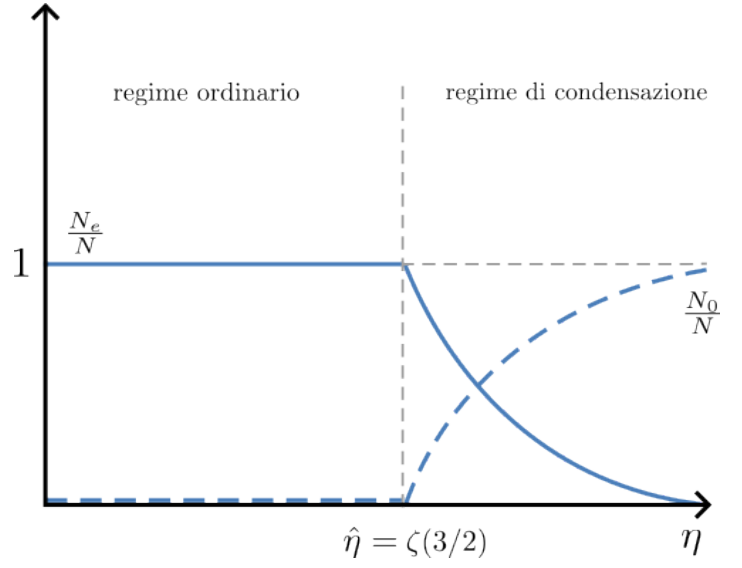
\includegraphics[width=0.5\linewidth]{Immagini/andamento di Ne (gas bosoni liberi).png}
        \caption{andamento di $N_e/N$ in funzione di $\eta$ per un gas di bosoni liberi.}
        \label{fig: andamento di Ne (gas bosoni liberi).}
    \end{figure}
    Anche se coesistono, la fase condensata tende a prevalere su quella normale al crescere di $\eta$, seguendo una transizione omogenea. La fugacità $z$ in questo regime si ottiene invertendo la definizione di $N_0$ ottenendo, considerandola nel limite termodinamico, che
    \begin{equation}
         z = \frac{N_0}{N_0 + 1} \to 1,\quad N_0 \to \infty,
    \end{equation}
    e il conseguente andamento in funzione di $\eta$ mostrato in figura \ref{fig: andamento di z (gas bosoni liberi)}. 
    \begin{figure}[h]
        \centering
        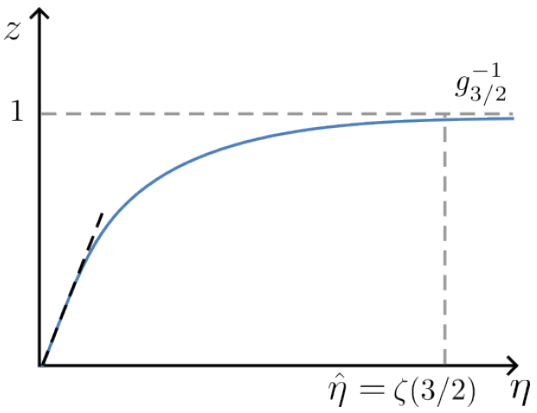
\includegraphics[width=0.45\linewidth]{Immagini/andamento di z (gas bosoni liberi).png}
        \caption{andamento di $z$ in funzione di $\eta$ per un gas di bosoni liberi.}
        \label{fig: andamento di z (gas bosoni liberi)}
    \end{figure}
    Ricordando l'espressione della pressione nella \eqref{eq: pressione e densità gas bosoni liberi (grancanonico)}, in questo regime $p$ si riduce al valore costante
    \begin{equation}
        p \simeq \frac{kT}{V_T}\zeta(5/2),
    \end{equation}
    mentre l'equazione di stato diventa
    \begin{equation}
        pV = kTN\frac{1}{\eta}\zeta(5/2),\quad \eta > \hateta \equiv \zeta(3/2),
    \end{equation}
    la quale al valore critico assume la forma
    \begin{equation}
        pV|_{\eta = \hateta} = kTN_e\frac{\zeta(5/2)}{\zeta(3/2)} \simeq 0.513 \times kTN,
    \end{equation}
    ossia lo stesso valore limite ottenibile nel regime usuale. Dunque, la quantità $pV/NkT$ è continua ovunque compreso nel punto critico $\hateta$, oltre il quale l'andamento segue un'iperbole come mostrato in figura \ref{fig: andamento pV (gas bosoni liberi)}.
    \begin{figure}[h]
        \centering
        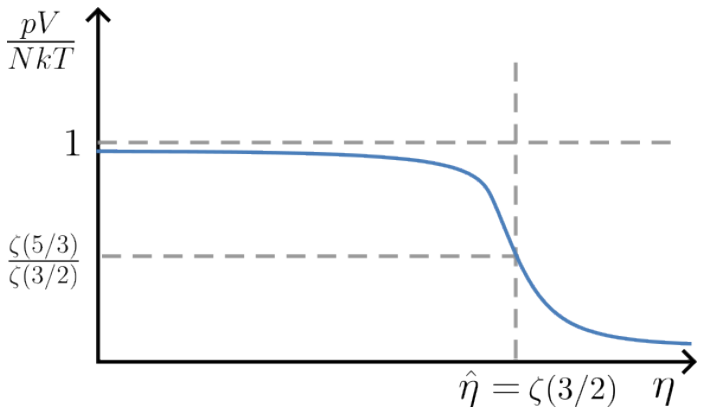
\includegraphics[width=0.5\linewidth]{Immagini/andamento pV (gas bosoni liberi).png}
        \caption{andamento di $pV/NkT$ in funzione di $\eta$ per un gas di bosoni liberi.}
        \label{fig: andamento pV (gas bosoni liberi)}
    \end{figure}
    Questo è anche l'andamento dell'energia interna per $\eta > \hateta$, infatti
    \begin{equation}
        E = \frac{3}{2}pV \simeq \frac{3}{2}kTN\frac{1}{\eta}\zeta(5/2),
    \end{equation}
    la quale può essere riscritta, usando la \eqref{eq: frazione bosoni eccitati bassa T (grancanonico)}, come
    \begin{equation}
        E =  \frac{3}{2}kTN_e\frac{\zeta(5/2)}{\zeta(3/2)}
    \end{equation}
    mostrando così come sia solo la fase `usuale'' a contribuire all'energia interna, dato che nella fase condensata tutte le componenti sono nel livello $\epsilon_0 = 0$: le componenti nello stato fondamentale non contribuiscono alla pressione, quindi quando la frazione di particelle nello stato eccitato diminuisce, diminuisce la pressione. Per quanto riguarda la capacità termica, considerando che $V_T = \lambda_T^3 \propto T^{-3/2}$ e $E\propto T^{5/2}$, questa è
    \begin{equation}
        c_{V,N} = \frac{3}{2}kN\frac{5}{2}\frac{1}{\eta}\zeta(5/2),
    \end{equation}
    la quale valutata nel punto critico diventa
    \begin{equation}
        c_{V,N}|_{\eta = \hateta} = \frac{3}{2}kN\frac{\zeta(5/2)}{\zeta(3/2)} \simeq 1.26\times\frac{3}{2}kN,
    \end{equation}
    che è il medesimo valore ottenibile dall'espansione viriale per $\eta \to \hateta^-$ nel regime usuale. Dunque, la capacità termica è continua rispetto al punto critico $\hateta$; tuttavia, il suo andamento in figura \ref{fig: andamento cap. termica (gas bosoni liberi)} mostra una cuspide proprio in $\hateta$ implicando che la derivata di $c_{V,N}$ è discontinua. 
    \begin{figure}[h]
        \centering
        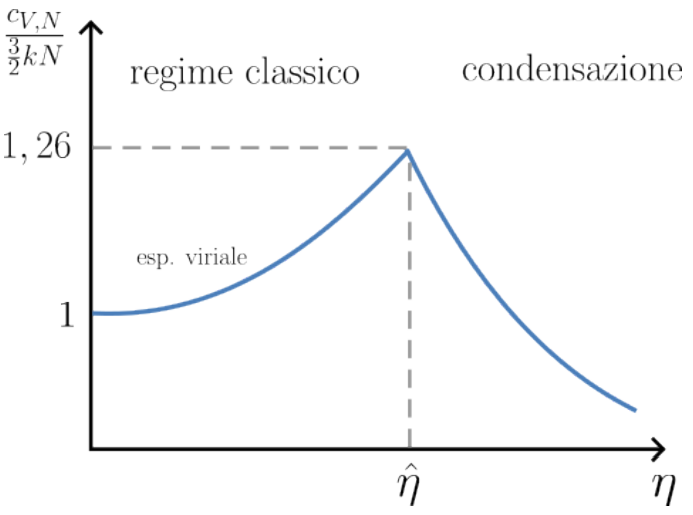
\includegraphics[width=0.45\linewidth]{Immagini/andamento cap. termica (gas bosoni liberi) 1.png}
        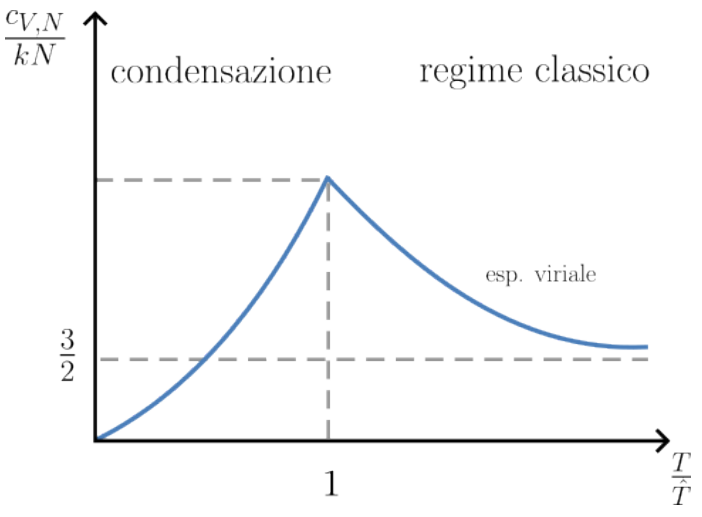
\includegraphics[width=0.45\linewidth]{Immagini/andamento cap. termica (gas bosoni liberi) 2.png}
        \caption{andamento di $3c_{V,N}/2kN$ per un gas di bosoni liberi in funzione di: (i) $\eta$; (ii) $T/\hatT$.}
        \label{fig: andamento cap. termica (gas bosoni liberi)}
    \end{figure}
    Spesso per il confronto con i dati sperimentali, si considera un sistema avente $N$ e $V$ fissati e ci si concentra sulla dipendenza da $T$ delle varie quantità termodinamiche. In particolare, si ha
    \begin{equation}
        \eta = \frac{V_T}{v} = \frac{\lambda_T^3}{v} = cT^{-3/2},\quad c = \frac{1}{v}\bigg(\frac{h^2}{2\pi mk}\bigg)^{3/2}.
    \end{equation}
    Il valore critico $\hateta$ individua la temperatura critica $\hatT$ tramite
    \begin{equation}
        \zeta(3/2) \equiv \hateta = c\hatT^{-3/2}\quad\Longrightarrow\quad c = \zeta(3/2)\hatT^{3/2},
    \end{equation}
    per cui si può scrivere 
    \begin{equation}
        \eta = \bigg(\frac{\hatT}{T}\bigg)^{3/2}\zeta(3/2),
    \end{equation}
    ottenendo il grafico dell'andamento di $c_{V,N}/kN(\hatT/T)$ sempre in figura \ref{fig: andamento cap. termica (gas bosoni liberi)}. Questo andamento è qualitativamente molto simile al grafico del calore specifico dell'$\ce{^4He}$ liquido. Nel 1938 London suggerì che questa singolarità per $T \simeq \SI{2.19}{\kelvin}$ fosse spiegabile in termini della condensazione di Bose - Einstein. In effetti, se si sostituiscono nella i valori appropriati di massa e volume molare dell'$\ce{^4He}$ nella \eqref{eq: temperatura critica gas di bosoni (grancanonico)} si ottiene
    \begin{equation}
        \hatT \simeq \SI{3.13}{\kelvin}.
    \end{equation}
    L'interpretazione di questa transizione dell'elio liquido come condensazione di Bose - Einstein è in accordo con il modello empirico semi-fenomenologico di Tisza basato sul fatto che le caratteristiche di una transizione di questo tipo dovessero corrispondere alla coesistenza di due fasi fluide diverse. Le due fasi sono quelle ``normale'' e quella ``condensata'' che compare per $T = \hatT$ e diviene dominante con il diminuire di $T$.
\end{caso}

\subsection{Gas di fotoni}
Si consideri una cavità di volume $V$ le cui componenti sono mantenute a temperatura costante $T$, al cui interno è intrappolata della radiazione elettromagnetica. Dato che si sta parlando di particelle a massa nulla, la situazione è leggermente diversa da quella dei bosoni liberi studiati precedentemente, quindi non si rientra nella condensazione di Bose - Einstein. Nella prospettiva dell'Elettrodinamica quantistica si ha un gas di quanti del campo elettromagnetico, i fotoni possono essere creati o annichilati nelle interazioni con la materia delle pareti: il loro numero non è fisso e non c'è costo energetico nel variarlo. Dunque, il potenziale
chimico è nullo $\mu = 0$ e per la dualità onda-particella l'energia di ogni singolo fotone è $\epsilon = \hbar\omega$. La conseguente relazione di dispersione è $\omega = c|\vk| \equiv ck$. Inoltre, il fotone possiede due stati di elicità dati da $\pm\hbar$ che corrispondono alle due possibili polarizzazioni trasverse indipendenti dalle onde elettromagnetiche, quindi $g_s = 2$ e la degenerazione dei fotoni con la stessa energia è data da
\begin{equation}
    g(\omega) = \frac{2V}{2\pi^2c^3}\omega^2 = \frac{V}{\pi^2c^3}\omega^2.
\end{equation}
Il potenziale grancanonico $\varpi_B$ per un gas ideale di bosoni liberi, nel caso del gas di fotoni, diventa
\begin{equation}
    \varpi = kT\int_0^\infty d\omega\,g(\omega)\log{(1 - e^{-\beta\hbar\omega})} = \frac{kTV}{\pi^2c^3}\int_0^\infty d\omega\,\omega^2\log{(1 - e^{-\beta\hbar\omega})},
\end{equation}
da cui si possono derivare le quantità termodinamiche di interesse. Partendo dalla pressione, questa è data da
\begin{equation}
    p = -\frac{\varpi}{V} = \frac{kT}{\pi^2c^3}\int_0^\infty d\omega\,\omega^2\log{(1 - e^{-\beta\hbar\omega})},
\end{equation}
che integrata per parti, considerando l'annullamento dei termini al bordo e cambiando variabile con $x = \beta\hbar\omega$, diventa
\begin{equation}
    \begin{split}
        p = -\frac{kT}{\pi^2c^3}\int_0^\infty\frac{d(\omega^3)}{3}\log{(1 - e^{-\beta\hbar\omega})} &= \frac{kT}{3\pi^2c^3}\int_0^\infty d\omega\,\omega^3\frac{\beta\hbar e^{-\beta\hbar\omega}}{1 - e^{-\beta\hbar\omega}} \\
        &\overset{x=\beta\hbar\omega}{=} \frac{k^4T^4}{3\pi^2c^3\hbar^3}\int_0^\infty dx\,\frac{x^3e^{-x}}{1 - e^{-x}}.
    \end{split}
\end{equation}
Adesso ricordando il risultato ottenuto per la costante di Debye in \eqref{eq: costante di Debye}, si ha che la pressione del gas di fotoni è
\begin{equation}
\label{eq: pressione gas di fotoni}
    p = \frac{\pi^2k^4}{45c^3\hbar^3}T^4 = \frac{4}{3c}\sigma T^4,\quad \sigma = \frac{\pi^2k^4}{60c^2\hbar^3} \simeq \SI{5.67}{\joule\meter^{-2}\second^{-1}\kelvin^{-4}},
\end{equation}
dove la costante di proporzionalità $\sigma$ prende il nome di ``costante di Stefan - Boltzmann''. Quindi, l'energia interna è ottenuta come al solito ma considerando che adesso $\mu = 0$, per cui
\begin{equation}
    \begin{split}
        \vmedio{E} = \frac{\p(\beta\varpi)}{\p\beta}\bigg|_{N,\mu = 0} &= \frac{V}{\pi^2c^3}\int_0^\infty d\omega\,\omega^2\frac{\p}{\p\beta}\log{(1 - e^{-\beta\hbar\omega})} \\
        &= \frac{V}{\pi^2c^3}\int_0^\infty d\omega\,\omega^2\hbar\omega\frac{e^{-\beta\hbar\omega}}{1 - e^{-\beta\hbar\omega}},
    \end{split}
\end{equation}
che in termini della pressione può essere espressa come
\begin{equation}
    \vmedio{E} = 3pV.
\end{equation}
Inoltre, si può scrivere la densità di energia totale come
\begin{equation}
    \frac{\vmedio{E}}{V} = \int_0^\infty d\omega\,\rho(\omega),
\end{equation}
dove $\rho(\omega)$ rappresenta la densità di energia per unità di frequenza ed è data dalla legge di Planck della radiazione
\begin{equation}
    \rho(\omega) = \frac{\omega^2}{\pi^2c^3}\frac{\hbar\omega}{e^{\beta\hbar\omega} - 1}.
\end{equation}
Quindi la densità di energia totale all'interno del corpo nero è distribuita in onde di frequenza diversa. Pertanto, ci si può chiedere quale sia la densità di energia presenta all'interno del corpo nero a seconda della frequenza. In realtà, nella pratica non si misura direttamente la densità di energia all'interno del corpo nero, ma si studia la radiazione emessa da esso; in particolare, si può mostrare che il flusso di energia per unità di frequenza e di superficie di un foro nella cavità è dato da
\begin{equation}
    I(\omega) = \frac{c}{4}\rho(\omega).
\end{equation}
Si definisce anche l'``emissività'' $\mathcal{E}$ di un corpo come l'intensità di tale energia emessa per unità di superficie 
\begin{equation}
    \mathcal{E} := \int_0^\infty d\omega\,I(\omega) = \frac{c}{4}\frac{\vmedio{E}}{V} = \sigma T^4,
\end{equation}
permettendo la derivazione sperimentale della costante di Stefan - Boltzmann.

Dato che il numero medio di fotoni può variare, allora è lecito chiedersi quale sia il valore medio del numero di fotoni $\vmedio{N}$. Questo si può calcolare dalla \eqref{eq: numero medio N (grancanonico)}, ponendo $z = 1$ e $\mu = 0$, adattando la definizione al continuo
\begin{equation}
    \vmedio{N} = \frac{V}{\pi^2c^3}\int_0^\infty d\omega\,\omega^2\frac{1}{e^{\beta\hbar\omega} - 1} \equiv V\int_0^\infty d\omega\, u(\omega),
\end{equation}
dove si è definita la densità di fotoni per unità di frequenza come
\begin{equation}
    u(\omega) = \frac{\omega^2}{\pi^2c^3}\frac{1}{e^{\beta\hbar\omega} - 1},
\end{equation}
la quale è direttamente collegata alla densità di energia per unità di frequenza tramite $\rho(\omega) = \hbar\omega u(\omega)$, dato che ogni fotone contribuisce con un quanto di energia $\epsilon = \hbar\omega$. Operando poi il cambio di variabile $x = \beta\hbar\omega$, si ottiene
\begin{equation}
    \frac{\vmedio{N}}{V} = \frac{k^3T^3}{\pi^2c^3\hbar^3}\int_0^\infty dx\,\frac{x^2}{e^x - 1} \equiv \frac{k^3T^3}{\pi^2c^3\hbar^3}J,
\end{equation}
dove l'integrale $J$ può essere valutato in un modo analogo a quanto fatto per calcolare la costante di Debye in \eqref{eq: costante di Debye} tramite l'espansione in serie geometrica ottenendo
\begin{equation}
     J = \Gamma(3)\zeta(3) = 2\zeta(3) \simeq 2.401.
\end{equation}
Dunque, la densità media dei fotoni è
\begin{equation}
\label{eq: densità gas di fotoni}
    \frac{\vmedio{N}}{V} = 2\zeta(3)\frac{k^3T^3}{\pi^2c^3\hbar^3}.
\end{equation}
Sfruttando infine la formula della pressione \eqref{eq: pressione gas di fotoni} in combinazione con la relazione appena trovata per la densità \eqref{eq: densità gas di fotoni} si ottiene l'equazione di stato meccanica nella forma
\begin{equation}
    pV = \frac{\zeta(4)}{\zeta(3)}\vmedio{N}kT \simeq 0.9003\times \vmedio{N}kT.
\end{equation}
Dunque, l'equazione di stato meccanica non corrisponde a quella classica, ma è corretta da un fattore moltiplicativo pari a circa $0.9003$.

\section{Gas classico interagente}
Fino ad ora si sono considerati solamente sistemi non interagenti, in cui l'energia è additiva nei contributi delle varie componenti, e si sono visti emergere effetti di interazione di tipo statistico nei sistemi quantistici che si creano quando le componenti sono indistinguibili. Tuttavia, non si sono mai considerate situazioni con termini di interazione presenti sin dall'inizio nell'hamiltoniana microscopica. In molte situazioni i termini di interazione sono ``piccoli'', come nel caso di un gas nel limite di alta temperatura o, equivalentemente, di bassa densità. In tal caso, si può procedere sistematicamente ad includere il loro effetto tramite una espansione perturbativa. Tale metodo, che storicamente precede quello analogo usato in Teoria dei campi, prende il nome di ``cluster expansion''. Per semplicità, ci si limita al primo ordine perturbativo, considerando un gas classico. 

Quindi, l'hamiltoniana di un sistema interagente ad $N$ componenti identiche di massa $m$ è
\begin{equation}
    H = \sum_{i=1}^N\frac{|\vp_i|^2}{2m} + \sum_{i < j}u_{ij}.
\end{equation}
Al proposito di seguire una trattazione perturbativa, si assume che le interazioni siano molto più ``piccole'' rispetto all'energia termica e che il potenziale di interazione dipenda unicamente dal modulo della distanza tra le componenti
\begin{equation}
    u_{ij} \equiv u(\vq_{ij}) = u(|\vq_i - \vq_j|).
\end{equation}
Se si tratta questo sistema classicamente, la funzione di partizione risulta essere
\begin{equation}
\label{eq: funzione di partizione sistema interagente (canonico)}
    \begin{split}
        Z_{(N)} &= \frac{1}{N!}\int\frac{d^{3N}p\,d^{3N}q}{h^{3N}}\,e^{-\beta H} \\
        &= \frac{1}{N!}\int\frac{d^{3N}p}{h^{3N}}\,e^{-\beta\sum_i|\vp_i|^2/2m}\int d^{3N}q\,e^{-\beta \sum_{i<j}u_{ij}} \\
        &\equiv \frac{1}{N!}\mathcal{P}(N)\mathcal{C}(N),
    \end{split}
\end{equation}
dove $\intp$ e $\intconfig$ sono rispettivamente gli integrali sui momenti e sulle coordinate, detto ``di configurazione''. In particolare, $\intconfig$ si può riscrivere come
\begin{equation}
    \intconfig = \int d^{3N}q\,\prod_{i<j}e^{-\beta u_{ij}},
\end{equation}
da cui si nota che, essendo l'integrando un esponenziale e quindi sempre positivo, allora anche $\intconfig \ge 0$. Chiaramente, nel caso ideale in assenza di interazioni, $u_{ij} = 0$ e quindi $\intconfig = \int d^{3N}q = V^N$. 

Adesso l'obiettivo è trovare un modo per organizzare $\intconfig$; nel caso interagente è conveniente introdurre una quantità che tenda a zero quando $\beta u_{ij}$ è ``piccolo'', consistentemente alle ipotesi assunte per il potenziale di interazione. Si definisce quindi
\begin{equation}
    f_{ij} := e^{-\beta u_{ij}} - 1 : \begin{cases}
        f_{ij} \to 0,\,\beta u_{ij} = 0 \\
        f_{ij} \ll 1,\,\beta u_{ij} \ll 1
    \end{cases}.
\end{equation}
L'espansione perturbativa pertanto non è altro che un'espansione per ``piccoli'' valori di $f$: Nel limite $\beta u_{ij} \ll 1$ è possibile espandere l'integrale di configurazione in potenze di $f$ come
\begin{equation}
    \intconfig = \int d^{3N}q\,\prod_{i<j}(1 + f_{ij}) = \int d^{3N}q\,\bigg(1 + \sum f_{ij} + \sum f_{ij}f_{kl} + \cdots\bigg),
\end{equation}
dove le somme simboliche nell'integrando stanno a rappresentare i termini aventi una copia di $f$, due copie di $f$, e così via. Dal primo termine, non essendoci alcuna dipendenza da $f$, si ritrova il risultato del sistema non interagente; dopo il primo termine, compaiono le correzioni dovute all'interazione, i vari contributi di tale espansione possono venire rappresentati graficamente come
\begin{align}
    \circled{i} &\equiv \int d^3q_i = V, \\
    \circled{i} - \circled{j} &\equiv \int d^3q_i\,d^3q_j\,f_{ij} \\
    \circled{i} - \circled{j} - \circled{k} &\equiv \int d^3q_i\,d^3q_j\,d^3q_k\,f_{ij}f_{jk}.
\end{align}
I grafici connessi prendono il nome di ``clusters'', da qui il nome ``cluster expansion'' del metodo. Limitandosi ai cluster di secondo ordine, ossia al primo ordine non banale, si ha
\begin{equation}
    \begin{split}
        \intconfig &\simeq \int d^{3N}q + \sum_{i<j}\int d^{3(N-2)}q\int d^3q_i\,d^3q_j\,f_{ij} \\
        &= V^N + V^{N-2}\sum_{i<j}\int d^3q_i\,d^3q_j\,f_{ij},
    \end{split}
\end{equation}
che può essere scritto in termini di clusters osservando che le variabili $i$ e $j$ sono mute essendo integrate e quindi restituiscono il medesimo contributo per qualsiasi $f_{ij}$ permettendo di scegliere $i = 1$ e $j = 2$; quindi si ha
\begin{equation}
\label{eq: integrale di configurazione II ordine}
    \begin{split}
        \intconfig &\simeq V^N\bigg[1 + \binom{N}{2}\frac{1}{V^2}\int d^3q_1\,d^3q_2\,f_{12} \bigg] \\
        &= V^N\bigg[1 + \frac{N(N-1)}{2V^2}\circled{i}-\circled{j}\bigg].
    \end{split}
\end{equation}
Sostituendo l'espressione dell'integrale di configurazione \eqref{eq: integrale di configurazione II ordine} in quella della funzione di partizione \eqref{eq: funzione di partizione sistema interagente (canonico)} si ottiene
\begin{equation}
    Z_{(N)} = \frac{1}{N!}\bigg(\frac{V}{V_T}\bigg)^N\bigg[1 + \frac{N(N-1)V_T}{V}b_2 + \cdots\bigg],
\end{equation}
dove si sono definiti i coefficienti $b_i$, la cui forma è determinata unicamente da quella del potenziale di interazione $u_{ij}$; in particolare, per ragioni collegate all'organizzazione dei termini successivi, si pone
\begin{equation}
    b_2 := \frac{1}{2VV_T}\circled{i}-\circled{j}.
\end{equation}

Se si considerano anche le correzioni successive al primo ordine non banale, risulta sempre più conveniente passare all'enesemble grancanonico e definire la funzione di partizione grancanonica
\begin{equation}
    \begin{split}
        Q = \sum_{N=0}^\infty z^NZ_{(N)} &= \sum_{N=0}^\infty z^N\frac{1}{N!}\bigg(\frac{V}{V_T}\bigg)^N\bigg[1 + \frac{N(N-1)V_T}{V}b_2 + \cdots\bigg] \\
        &= \sum_{N=0}^\infty \frac{1}{N!}\bigg(\frac{zV}{V_T}\bigg)^N  + b_2\sum_{N=2}^\infty \frac{z^N}{(N-2)!}\bigg(\frac{V}{V_T}\bigg)^{N-1} + \cdots,
    \end{split}
\end{equation}
che all'ordine considerato coincide\footnote{Infatti, ricordando l'espansione in serie $e^x = \sum_{n=0}^\infty x^n/n!$, si ha
\begin{align}
        \exp{\bigg[\frac{zV}{V_T}(1 + b_2z + \cdots)\bigg]} &= \sum_{N=0}^{\infty} \frac{1}{N!} \bigg(\frac{zV}{V_T}\bigg)^N
        \bigg(1 + b_2 z + \cdots \bigg)^N \\
        &\simeq \sum_{N=0}^{\infty} \frac{1}{N!}
        \bigg(\frac{zV}{V_T}\bigg)^N
        \bigg(1 + N b_2 z + \cdots \bigg) \\
        &= \sum_{N=0}^{\infty} \frac{1}{N!} \bigg(\frac{zV}{V_T}\bigg)^N + b_2 \sum_{N=2}^{\infty}\frac{z^{N+1}}{(N-1)!} \bigg(\frac{V}{V_T}\bigg)^N + \cdots.
\end{align}
Per confrontare le due sommatorie, entrambe devono essere alla potenza $N$,
quindi si pone $M = N + 1$ nel secondo termine, cosicché 
\begin{align}
    \exp{\bigg[\frac{zV}{V_T}(1 + b_2z + \cdots)\bigg]} &= \sum_{N=0}^{\infty} \frac{1}{N!} \bigg(\frac{zV}{V_T}\bigg)^N + b_2 \sum_{M=2}^{\infty} \frac{z^M}{(M-2)!} \bigg(\frac{V}{V_T}\bigg)^{M-1} + \cdots = Q.
\end{align}} con
\begin{equation}
    Q = \exp{\bigg[\frac{zV}{V_T}(1 + b_2z + \cdots)\bigg]}.
\end{equation}
Dalla funzione di partizione si deduce il potenziale grancanonico 
\begin{equation}
    \varpi = -kT\log{Q} = -\frac{zVkT}{V_T}(1 + b_2z + \cdots),
\end{equation}
da cui a sua volta si deducono le quantità termodinamiche
\begin{align}
\label{eq: pressione e N medio gas interagente (grancanonico)}
    p &= -\frac{\varpi}{V} = \frac{zkT}{V_T}(1 + b_2z + \cdots), \\
    \vmedio{N} &= -\beta z\frac{\p\varpi}{\p z}\bigg|_{T,V} = \frac{V}{V_T}(z + 2b_2z^2 + \cdots).
\end{align}
Per ritornare alla trattazione canonica, si può semplicemente scrivere la relazione
\begin{equation}
    \eta \equiv \frac{\vmedio{N}}{V}V_T = z + 2b_2z^2 + \cdots
\end{equation}
che può essere invertita in
\begin{equation}
    z = \eta - 2b_2\eta^2 + \cdots,
\end{equation}
la quale sostituita nelle \eqref{eq: pressione e N medio gas interagente (grancanonico)} permette di scrivere l'equazione di stato come
\begin{equation}
    pV = kT\vmedio{N}(1 - b_2\eta + \cdots).
\end{equation}
In generale, considerando correzioni di ordine più alto, si ottiene l'espansione viriale
\begin{equation}
\label{eq: equazione di stato (espansione viriale)}
    pV = kT\vmedio{N}\sum_{l=1}^\infty a_l\eta^{l-1},
\end{equation}
dove gli $a_i$ sono i coefficienti viriali.
\begin{obs}
    Si può mostrare che il coefficiente $a_l$ è determinato dai clusters fino all'ordine $l$; per cui, se si decide di fermarsi ad un'ordine $l$ nella sommatoria, allora si considerano i cluster solo fino a quell'ordine.
\end{obs}
Dunque, si è trovato che l'effetto dell'interazione è quello di diminuire $pV$, perché tendono a formare stati legati e fare meno pressione. 

\subsection{Secondo coefficiente viriale}
L'obiettivo è calcolare il secondo coefficiente viriale $a_2$ dell'espansione \eqref{eq: equazione di stato (espansione viriale)} per un potenziale il cui andamento è mostrato in figura \ref{fig: potenziale coefficiente a2}. Un'espressione semi-empirica per potenziali di questo tipo è data dal potenziale di Lennard - Jones
\begin{equation}
\label{eq: potenziale Lennard-Jones}
    u(r_{ij}) = 4\epsilon\bigg[\bigg(\frac{\sigma}{r_{ij}}\bigg)^{12} - \bigg(\frac{\sigma}{r_{ij}}\bigg)^{6}\bigg],
\end{equation}
dove $\epsilon$ è l'energia associata al minimo del potenziale in $r_0 = 2^{1/6}\sigma$. In realtà, l'approssimazione che si usa qui è ancora più limitata, continuando però ad essere adatta all'ambito statistico. L'idea, mostrata in figura \ref{fig: potenziale coefficiente a2}, è quella di rimpiazzare la parte repulsiva del potenziale con un ``muro'' repulsivo
\begin{equation}
\label{eq: potenziale Lennard-Jones approx.}
    u(r_{ij}) = 
    \begin{cases}
        \infty,\, r < r_0\\
        u_0\bigg(\dfrac{r_0}{r_{ij}}\bigg)^6,\, r \ge r_0
    \end{cases}.
\end{equation}
Con questo specifico potenziale, il coefficiente $b_2$ risulta essere
\begin{equation}
    b_2 = \frac{1}{2VV_T}\circled{i}-\circled{j} = \frac{1}{2VV_T}\int d^3q_1\,d^3q_2\,f_{12}(r_{12}).
\end{equation}
\begin{figure}[h]
    \centering
    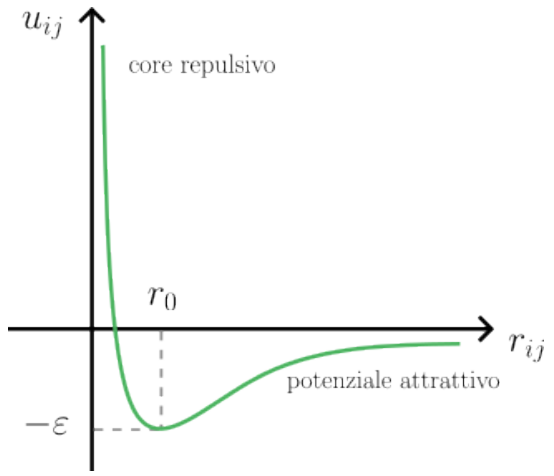
\includegraphics[width=0.4\linewidth]{Immagini/potenziale coefficiente a2.png}
    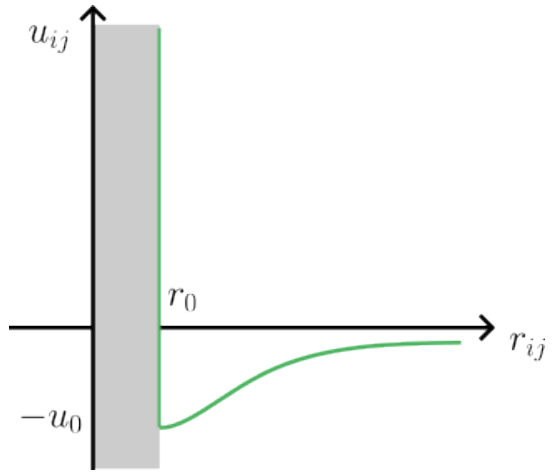
\includegraphics[width=0.4\linewidth]{Immagini/potenziale coefficiente a2 hardcore.png}
    \caption{potenziale intermolecolare di Lennard - Jones e la sua approssimazione ``hardcore''.}
    \label{fig: potenziale coefficiente a2}
\end{figure}
Dato che il potenziale dipende solo dalla distanza reciproca, allora è conveniente cambiare variabili in quelle del centro di massa avente jacobiano unitario
\begin{equation}
    \begin{cases}
        \vq_{CM} = \dfrac{1}{2}(\vq_1 + \vq_2) \\
        \vx = \vq_1 - \vq_2
    \end{cases},
\end{equation}
con le quali si ha
\begin{equation}
    \int d^3q_1\,d^3q_2\,f_{12}(r_{12}) = \int d^3q_{CM}\int d^3x\,f_{12}(|\vx|) = V\int d^3x\,f_{12}(|\vx|)
\end{equation}
e quindi, ricordando che la definizione $f_{ij} = e^{-\beta u_{ij}} - 1 $, si arriva a
\begin{equation}
    b_2 = \frac{V}{2VV_T}\int d^3x\,f_{12}(|\vx|) = \frac{1}{2V_T}\int d^3x\,[e^{-\beta u(|\vx|)} - 1].
\end{equation}
Passando adesso in coordinate in polari e tenendo conto della forma del potenziale \eqref{eq: potenziale Lennard-Jones approx.} si ha
\begin{equation}
    \begin{split}
        b_2 &= \frac{2\pi}{V_T}\int_0^\infty dr\,r^2[e^{-\beta u(r)} - 1] \\
        &= \frac{2\pi}{V_T}\bigg\{-\int_0^{r_0}dr\,r^2 + \int_{r_0}^\infty dr\,r^2[e^{\beta u_0(r_0/r)^6} - 1]\bigg\}.
    \end{split} 
\end{equation}
Per l'ipotesi sull'intensità dell'interazione $\beta u_{ij} \ll 1$, il secondo integrale è approssimare con
\begin{equation}
    e^{\beta u_0(r_0/r)^6} - 1 \simeq \beta u_0\bigg(\frac{r_0}{r}\bigg)^6,
\end{equation}
rimanendo con
\begin{equation}
\label{eq: coefficiente b2}
    \begin{split}
        b_2 &\simeq \frac{2\pi}{V_T}\bigg[-\frac{r_0^3}{3} + \beta u_0r_0^6\int_{r_0}^\infty \frac{dr}{r^4}\bigg] \\
        &= \frac{2\pi}{V_T}\bigg[-\frac{r_0^3}{3} - \frac{\beta u_0r_0^6}{3}\frac{1}{r^3}\bigg|_{r_0}^\infty\bigg] \\
        &= -\frac{2\pi}{3V_T}r_0^3(1 - \beta u_0).
    \end{split} 
\end{equation}
Sostituendo quanto ottenuto per $b_2$ in \eqref{eq: coefficiente b2} nell'equazione di stato \eqref{eq: equazione di stato (espansione viriale)}, tenendo conto che $a_2 = -b_2$, si trova la prima correzione viriale
\begin{equation}
\label{eq: equazione di stato (I corezione viriale)}
    pV \simeq kT\vmedio{N}\bigg[1 + \frac{2\pi r_0^3}{3v}\bigg(1 - \frac{u_0}{kT}\bigg)\bigg].
\end{equation}
Per quanto vi siano forti approssimazioni in questa derivazione, l'equazione di stato ottenuta è equivalente all'equazione di Van der Waals \eqref{eq: equazione di stato Van der Waals}, la quale è fenomenologicamente valida in questo regime. Infatti, si riscrive la \eqref{eq: equazione di stato (I corezione viriale)} come la relazione
\begin{equation}
    p + \frac{2\pi u_0r_0^3}{3v^2} = \frac{kT}{v}\bigg(1 + \frac{2\pi r_0^3}{3v}\bigg).
\end{equation}
Siccome si è considerato il limite di bassa densità, il volume disponibile $v$ per ogni particella deve essere molto più grande del volume escluso $r_0^3$, per cui si può dire che $r_0^3/v \ll 1$ e scrivere il secondo termine della relazione precedente come
\begin{equation}
    \bigg(1 - \frac{2\pi r_0^3}{3v}\bigg)^{-1} \simeq \frac{v}{v - 2\pi r_0^3/3},
\end{equation}
arrivando quindi a 
\begin{equation}
     \bigg(p + \frac{2\pi u_0r_0^3}{3v^2}\bigg)\bigg(v - \frac{2\pi r_0^3}{3}\bigg) = kT,
\end{equation}
che, ponendo $A \equiv 2\pi u_0r_0^3/3$ e $B \equiv 2\pi r_0^3/3$, coincide proprio con l'equazione di Van der Waals
\begin{equation}
    \bigg(p + \frac{a}{V^2}\bigg)(V - b) = NkT.
\end{equation}
\begin{obs}
    Nella \eqref{eq: equazione di stato Van der Waals} si era posto il numero di moli pari ad uno, per trovare un identico risultato basta definire $A = a/N^2$ e $B = b/N$.
\end{obs}
Si ricorda che l'interpretazione del parametro $B$ era quella di volume per particella ``escluso'' a causa del volume finito delle molecole. Effettivamente, anche ora compare il volume escluso $r_0^3$ che corrisponde ad una sfera di diametro $r_0$ e quindi di un volume
\begin{equation}
    \frac{4\pi}{3}\bigg(\frac{r_0}{2}\bigg)^3 = \frac{B}{4}.
\end{equation}
Il parametro $A$ era attribuito all'effetto dell'interazione attrattiva, e questo è confermato dalla proporzionalità con $u_0$. L'equazione di Van der Waals è dunque ottenuta da un'espansione perturbativa al primo ordine, quindi è valida solo nel limite di alte temperature. Se si volesse studiare il limite a basse temperature si dovrebbero incorporare correzioni successive che modificherebbero l'equazione di stato, che alla fine dovrebbe mostrare addirittura una transizione di fase. Quindi, quando le interazioni diventano rilevanti rispetto all'energia termica $kT$, l'equazione di Van der Waals non è più giustificata. Ecco perché questa equazione porta a conclusioni non fisicamente accettabili al di sotto di una temperatura critica; in particolare, viene violata la condizione di stabilità
\begin{equation}
    \frac{\p p}{\p V}\bigg|_{T,N} \le 0,
\end{equation}
che, con la costruzione di Maxwell, corrisponde alla comparsa di una transizione di fase. Questa non può venire catturata semplicemente da un'espansione perturbativa, nemmeno andando ad ordini più alti nell'espansione. Per ricavare esplicitamente le transizioni di fase dalla descrizione della Meccanica statistica sono necessarie soluzioni esatte, o quanto meno metodi non perturbativi. I primi risultati importanti riguardo alla spiegazione delle transizioni di fase furono ottenuti nell'ambito delle transizioni ferromagnetiche, con il modello di Ising.